% this is a modular LaTeX document. Please learn about it at these links:
% https://tex.stackexchange.com/questions/246/when-should-i-use-input-vs-include
% https://en.wikibooks.org/wiki/LaTeX/Modular_Documents

\documentclass[a4paper,12pt]{report}
%\usepackage[a4paper,inner=1.7cm, outer=2.7cm, top=2cm, bottom=2cm, bindingoffset=1.2cm]{geometry} 
\usepackage[english]{babel} % use the english babel package. 
\usepackage[scaled=.92]{helvet} % tells you to use the helvetica font. 

% Graphics Packages and Declarations
\usepackage{graphicx} % allows you to use pictures in your document.
\usepackage{caption} % allows you to have captions
\usepackage{subcaption} % allows you to use subcaptions and subgraphics.
\usepackage{wrapfig} % allows you to wrap text around your picture.
 \usepackage{pdfpages} 
\graphicspath{{"C:/Users/LocalAdmin/Desktop/LaTeX Master Thesis/graphics"}}
%\graphicspath{ 	{C:/Users/LocalAdmin/Desktop/LaTeX Master Thesis/graphics} %main graphics path
			%{C:/Users/LocalAdmin/Desktop/LaTeX Master Thesis } % main path
			%{C:/Users/LocalAdmin/Desktop/LaTeX Master Thesis/graphics/tsmppt_troubleshooting} % MS view path
		%}
%\DeclareGraphicsExtensions{.eps,.png,.pdf}


\usepackage{enumitem}% have your lists look nicer.
%\usepackage{fancyhdr} % allows you to have nice looking headers.
\usepackage{amsmath} % allows you to write math formula.
\usepackage{index} % allows you to use indexes that are automatically generated.
\usepackage{hyperref} % allows you to insert hyperlinks.
\usepackage{gensymb} % allows you to use symbols. 
% makes an index.
\makeindex


% this is the actual environment.
\begin{document}
%title, author, and date specifications

\title{\Large{\textbf{Senior Thesis}}}
\author{By William Kerr}
\iffalse
\date{\date{\parbox{\linewidth}{\centering%
  \today\endgraf\bigskip
  Coordinator 1 \hspace*{3cm} Coordinator 2\endgraf\medskip
  Dept.\ of Physics \endgraf
  ABC College}}}
\fi
\maketitle % Automatically generates the title page.
\tableofcontents %Automatically generates a table of contents page.

%metadata
% page numbering data
\pagenumbering{roman} %sets page numbering style to "roman numerals"
\setcounter{page}{2} % start page numbering on page 2.

% header data
%\fancyhf{} % clear default headers.
%\renewcommand{\headrulewidth}{2pt} % redefine headrulewidth to 2pt.
%\renewcommand{\footrulewidth}{1pt} % redefine footrulewdith to 1pt. (make it different)
%\fancyhead[LE]{\leftmark} % show the left makr on the Left side of hte page.
%\fancyhead[RO]{\nouppercase{\rightmark}} % on the right side of the page, display the chapter name.
%\fancyfoot[LE,RO]{\thepage} % just show the page number. 

\chapter{Abstract}
Lorem Ipsum 
\chapter{Introduction}% start a new chapter.

Per Previous Teams:
\newline
The University of California, Santa Cruz’s Arboretum has a very neglected
micro-grid with practically non-existent management. This has enabled reconfiguration
by those who don’t understand the intricacies of their actions, and
hence encourages increasing complexity of the system. The grid itself is in a
terrible state of disarray, featuring unfortunate developments such as random,
hanging live wires, batteries more than 5 years expired, inadequate power for
more crucial items, and plenty of broken equipment with obfuscated wiring,
that still sit in the same housing as the working equipment. We are the team
tasked with amending this poor facility’s design once and for all, with great
advancements such as a completely new design, fool-proof safety, and guidelines
for future expansion. We hope this document elaborates on the dire need to
make changes to the grid as well as documents what changes we recommend
and plan to implement.
\newline

The monitoring project is part of the greenhouse research facility at the University of California, Santa
Cruz which aims to provide an interactive electrical system for producing successful harvests. It is an
ongoing project that is in its second iteration, 2017-18’, with the goal of remotely monitoring and
regulating the greenhouse environmental conditions. The client’s needs are to create a plug-n-play
metering hub and web interface for students to conduct horticulture experiments using solar energy.
This year’s productivity involved gathering old documentation, revamping the server, developing a usermanual,
and creating a website. The ability to monitor the electrical grid through serial communication
was researched, forwarded, and documented. To complete the prototype of the metering system there
must be power-data analytics on the website along with charts and graphs of conditions. This document
serves to assist in understanding the current state of the system and for future work.


% the \input{} command includes a tex file into this main.text file.
% this makes this document modular, so I don't have to maintain it as much as a single gigantic file.

\chapter{Components Section}
\section{Solar Panels}
% adapted from the MS word document.
\subsection{Introduction}

This is a client request. These solar panels let certain wavelengths of light through them, and absorb the rest of the spectrum. This allows plants to grow inside.

\subsection{Data}
Model: LUMO 20M100GH \\
Quantity: 24x \\
Company: Soliculture \\
Company Website: \href{http://www.soliculture.com/}{http://www.soliculture.com/} \\
Product Page: \href{http://www.soliculture.com/product/}{http://www.soliculture.com/} \\

\subsection{Datasheet}
todo
 
\section{Charge Controller}
\subsection{Introduction}

Solar panels cannot charge batteries directly for these reasons: 
\begin{itemize}
	\item They have unstable voltages, and thus should not be connected directly to the battery. 
	\item Batteries with different chemical compositions charge differently. 
	\item One solar panel cannot provide enough power to the battery alone, even if it reaches the nominal voltage of 12V. 
	\item If we string 12 solar panels in series together and plug it into the batteries, the batteries will become permanently damaged.
\end{itemize}

Solar panels cannot charge batteries properly by themselves. We must have a charge controller to accompany the solar panels in order to charge the batteries properly. I like the TS-MPPT-60 because it is custom-programmable, and it can monitor a significant amount of values that could be useful someday. I included the values it can monitor below.

\subsection{Data}
Model: MORNINGSTAR TS-MPPT-60 TriStar MPPT 150V\\
Company: Morningstar\\
Company Website: \href{https://www.morningstarcorp.com}{https://www.morningstarcorp.com}\\
Product link: \href{https://www.morningstarcorp.com/products/tristar-mppt/}{https://www.morningstarcorp.com/products/tristar-mppt/}\\
Quantity: 2x\\
\subsubsection{Features}
\begin{itemize}
	\item Customizable Charge Settings
	\item Great networking capabilities
	\item RS-232 electrical interface for Microcontroller communication.
	\item Uses royalty-free MODBUS protocol for easy data harvesting
	\item Operating Range: -40\degree C to 40\degree C
	\item Up to 60A continuous battery current
	\item Compatible with 12V, 24V, and 48V battery systems
	\item Maximum 150V solar panels in series
	\item Keyholes for mounting
	\item Uses TrakStar MPPT technology to track the maximum power point of the solar panels.
	\item Temperature compensation
	\item Two Tristar Morningstar MPPT’s can be attached to the same battery pack
\end{itemize}

\subsubsection{Drawbacks}

The internal PLC settings can only be changed with a PC that can run MSView, Morningstar’s proprietary program that can program any Morningstar device, that can be downloaded from Morningstar’s website, located here:\\

\href{https://www.morningstarcorp.com/msview/}{https://www.morningstarcorp.com/msview/}\\

It can only handle 150V of solar panels. We have 24 solar panels, which in series total to a nominal voltage of 192V. Therefore, we must have at least 2.


\subsection{Monitoring}

A Tristar Morningstar MPPT can monitor these variables:

\paragraph{Internal ADC chips}


\begin{itemize}
	\item Battery Voltage
	\item Battery Terminal Voltage
	\item Battery Sense Voltage
	\item Array Voltage (of the solar panels)
	\item Battery Current
	\item Array Current (of the solar panels)
	\item 12V supply
	\item 3V supply
	\item meterbus voltage
	\item 1.8V supply
	\item Reference voltage
\end{itemize}
\par
\paragraph{Temperature Data}
\begin{itemize}
	\item Heatsink Temperature
	\item RTS temperature
	\item Battery Regulation Temperature
\end{itemize}
\par 

\paragraph{Status Data}
\begin{itemize}
	\item Battery Voltage (slow)
	\item Charging Current (slow)
	\item Minimum Battery Voltage
	\item Maximum Battery Voltage
	\item Hourmeter
	\item Faults raised
	\item Alarms raised
	\item LED state
	\item DIP switch status
\end{itemize}
\par

\paragraph{MPPT Data}
\begin{itemize}
	\item Output Power
	\item Input Power
	\item Max power of last sweep
	\item Vmp of last sweep
	\item Voc of last sweep
\end{itemize}
\par

\paragraph{Charger Data}
\begin{itemize}
	\item Charge state
	\item Target Regulation Voltage
	\item Ah charge resettable:
	\item Ah charge total
	\item kWhr charge resettable
	\item kWhr charge total
\end{itemize}
\par

\paragraph{Daily Data}
\begin{itemize}
	\item Battery Voltage Minimum
	\item Battery Voltage Maximum
	\item Input Voltage Maximum
	\item Amp Hours accumulated
	\item Watt hours accumulated
	\item Minimum Power output
	\item Minimum temperature
	\item Maximum temperature
	\item Time in equalize stage
	\item Time in float stage
	\item Alarms of the day
	\item Faults of the day
	\item Flags of the day
\end{itemize}
\par

\paragraph{Current Charge Settings}
\begin{itemize}
	\item EV\_absorp
	\item EV\_float
	\item Et\_absorp
	\item Et\_absorp\_ext
	\item EV\_absorp\_ext
	\item EV\_float\_cancel
	\item Et\_float\_exit\_cum
	\item EV\_eq
	\item Et\_eqcalendar
	\item Et\_eq\_above
	\item Et\_eq\_reg
	\item Et\_battery\_service
	\item EV\_tempcomp
	\item EV\_hvd
	\item EV\_hvr
	\item Evb\_ref\_lim
	\item ETb\_max
	\item Etb\_min
	\item Elb\_lim
	\item EVa\_ref\_fixed\_init
	\item EVa\_ref\_fixed\_pet\_init
\end{itemize}
\par

\paragraph{LED settings}
\begin{itemize}
	\item EV\_soc\_g\_gy
	\item EV\_soc\_gy\_y
	\item EV\_soc\_y\_yr
	\item EV\_soc\_yr\_r
\end{itemize}
\par

\subsection{Recommended Accessories}

\subsubsection{Remote Temperature Sensor}

\paragraph{Introduction}

The greenhouse will naturally change temperature more than 5 C during the year. The Morningstar Corporation recommends that you add the RTS sensor for the Charge Controller to operate more effectively under these circumstances. It is simple to install. Follow Morningstar’s guide to installation.\\
\\
Model: Remote Temperature Sensor\\
Quantity: 2x\\
Company: Morningstar\\
Company Website: \href{https://www.morningstarcorp.com/}{https://www.morningstarcorp.com/}\\
Product Page: \href{https://www.morningstarcorp.com/products/remote-temperature-sensor/}{https://www.morningstarcorp.com/products/remote-temperature-sensor/
}
\par

\subsubsection{RS-232 to USB cable}

\paragraph{Introduction}

RS-232 must be converted to USB format for easy monitoring by the Raspberry Pi. Luckily, I don’t have to reinvent the wheel. I can simply use this cable. It has an FTDI chip and board embedded inside the plug, so I don’t have to worry about fabricating a chip.\\
 \\
I’m going with a USB terminal because my microcontroller is a Raspberry Pi, and it’s simpler to use a USB and create a virtual COM port inside the Raspberry Pi’s Linux operating system.\\
 \\
Model: C2G 26886 USB to DB9 Serial RS232 Adapter Cable, Blue (1.5 Feet, 0.45 Meters)\\
Quantity: 2x\\
Company: C2G\\
Company Website: \href{https://www.cablestogo.com/}{https://www.cablestogo.com/} \\
Product Page: \href{https://www.amazon.com/C2G-Cables-26886-Serial-Adapter/dp/B000067RVJ}{https://www.amazon.com/C2G-Cables-26886-Serial-Adapter/dp/B000067RVJ}

\par

\section{Batteries}

\subsection{Lithium-ion Battery Cell}

\subsubsection{Introduction}

Solar panels do not produce power all the time. Even when they do produce power, they often don’t produce enough power to satisfy the consumer. During the day, when the solar panels produce the most power, the consumer often isn’t using the system. To resolve this, we need to have a battery pack. During the day, the battery pack will be charged by the solar panels, and during the evening, the battery pack will be discharged by the consumer.\\
 \\
Model: IFP71/180/278-CA180FI\\
Quantity: 8\\
Company:  CALB
Company website: \href{http://www.calbusainc.com/}{http://www.calbusainc.com/}
Product Page: \href{https://www.ev-power.eu/LiFePO4-small-cells/Prismatic/CALB-CA180FI-Lithium-Cell-LiFePO4-3-2V-180Ah.html}{ https://www.ev-power.eu/LiFePO4-small-cells/Prismatic/CALB-CA180FI-Lithium-Cell-LiFePO4-3-2V-180Ah.html}

\subsubsection{Datasheet}
TODO

\section{Battery Management System}

\subsection{Introduction}
Batteries don’t discharge evenly. Every battery has its own individual chemistry due to imperfections in the manufacturing process. If we discharge batteries unevenly, one battery could be worn out while another battery remains untouched. To resolve this, we use a Battery Management System.\\

\subsection{Main Controller}

Model: G1 EMUS BMS control unit\\
Quantity: 1\\
Company: Emus\\
Company Website: \href{https://emusbms.com/}{https://emusbms.com/} \\
Product Page: \href{https://emusbms.com/product/g1-bms-control-unit}{https://emusbms.com/product/g1-bms-control-unit} \\

\subsection{Features}
Automatically controls the battery operation process utilizing various interfaces for measurement, control, data exchange, configuration and indication, and works with any charge controller.
\paragraph{Application}
\begin{itemize}
	\item Any lithium chemistry, series connected battery pack of up to 254 cells if using serial cell communication
	\item Any lithium chemistry, series connected battery pack, or pack of multiple parallel strings, up to 8128 cells total, if using EMUS CAN Cell Group Modules.
	\item Storage Temperature: -40\degree C to 95\degree C
	\item Operation Temperature: -40\degree C to 80\degree C
	\item USB interface for Microcontroller reading
	\item Proprietary serial interface for cell communication
\end{itemize}

\subsection{Monitoring}

BMS control unit can monitor:

\subsubsection{System Status}
\begin{itemize}
	\item Battery Charge
	\item Charger Status
	\item Current and Voltage
	\item Distance and Energy (if applied to an electric vehicle)
	\item BMS status
	\item Time and Date
	\item Version Number
\end{itemize}

\subsubsection{System status and Individual Cells}
\begin{itemize}
	\item Battery Balancing Rate
	\item Temperature
	\item Battery Voltage
\end{itemize}

\subsubsection{Statistics}
Has an internal events log (each event happening at a recorded time)

Has a statistics log at a recorded time. Possible statistics to log:
\begin{itemize}
	\item Total Discharge
	\item Total Charge
	\item Total Discharge Energy
	\item Total Charge Energy
	\item Total Discharge Time
	\item Total Charge Time
	\item Total Distance
	\item Max Discharge Current
	\item Max Charge Current
	\item Min Cell Voltage
	\item Max Cell Voltage
	\item Max cell Voltage Difference
	\item Min pack voltage
	\item Max pack voltage
	\item Min Cell Module Temperature
	\item Max Cell Module Temperature
	\item Max Cell Module Temperature Difference
	\item Protection Counts (undervoltage, overvoltage, discharge overcurrent, charge overcurrent, cell module overheat, leakage protection, no cell communication, low voltage power reduction, high current power reduction, high cell module temperature power reduction, charger connect, charger disconnect, cell overheat, high cell module temperature power reduction)
	\item Miscellaneous counts (number of Preheat stages, Precharge stages, main charge stages, balancing stages, charging finished stages, charging errors, charging retries, trips, charge restarts)
	\item Min Cell Temperature
	\item Max Cell Temperature
	\item Max Cell Temperature Difference
\end{itemize}
\subsection{Necessary Accessories}

\subsubsection{Cell Isolators}

The BMS system requires that you have isolators to protect the main module. Only works if only 1 group of batteries is used.
 \\
Model: G1 Top/Bottom Isolator\\
Company Website: \href{https://emusbms.com/}{https://emusbms.com/} \\
Product Page: \href{https://emusbms.com/product/g1-top-bot-isolator}{https://emusbms.com/product/g1-top-bot-isolator} \\
Quantity: 2x \\

\subsubsection{Cell Modules}

Every battery must have its own cell module. Different batteries require different cell modules.You can find all types of cell modules here:
 \\
\href{https://emusbms.com/product-category/cell_modules}{https://emusbms.com/product-category/cell\_modules}
 \\
The standard solution is the A/B type, so that’s what we’re going with.We must order this package for each battery.

\paragraph{Ordering Schematic}
EMUS BMS Cell Module A – 1x
EMUS BMS Cell Module B – 1x
Ring Terminal M8 – 2x
Communication Cable – 16cm – 2x
\par
\paragraph{Ordering details}

Model: G1 Cell Module – A/B type\\
Company: Emus\\
Company Website: \href{https://emusbms.com}{https://emusbms.com/} \\
Product Page: \href{https://emusbms.com/product/g1-cell-module-ab}{https://emusbms.com/product/g1-cell-module-ab} \\
Quantity: 8x \\

\subsubsection{CAN Cell Group Module}

We need to group batteries into groups.
Since the batteries we picked are 3.2V, we group batteries into groups of 4.  
 \\
Model: G1 CAN Cell Group Module\\
Company: Emus \\
Company Website: https://emusbms.com/ \\
Product Page: https://emusbms.com/product/g1-can-cell-group-module \\
Quantity: 2x\\


\subsection{Recommended Accessories}

\subsubsection{Current Sensor}

In order to monitor current dispensing from the batteries to the load, you must have a current sensor. It’s not necessary for operation, but it’s recommended to have one. This one works using the hall effect, so it does not require contact with the wires; it only needs to have the wire running through its hole. \\
 \\
Model: G1 Loop Style Dual Range Current Sensor\\
Company: Emus \\
Company Website: \href{https://emusbms.com/}{https://emusbms.com/}
Product Page: \href{https://emusbms.com/product/g1-loop-style-dual-range-current-sensor}{https://emusbms.com/product/g1-loop-style-dual-range-current-sensor}\\
Quantity: 1x \\



 
\section{Sensors – Faculty}
\subsection{Introduction}
The client wants their own sensors exclusive for faculty. They want to measure temperature, humidity, and light. I propose that we use these classes of sensors for this:\\
\begin{itemize}
	\item Temperature and Humidity Sensor
	\item Light Sensor
\end{itemize}
The product page for the parts and their respective datasheets will be hosted by different companies. This is because it is easier to order a breakout board than it is to order the individual parts, order a custom PCB for the sensor, and solder the parts onto the board. Companies that sell breakout boards and companies that manufacture parts are separate from one another.

\subsection{Temperature and Humidity Sensor}
Model: BME280 \\
Company: Bosch \\
Company Website: \href{https://bosch.us/}{https://bosch.us} \\
Product Page: \href{https://www.adafruit.com/product/2652}{https://www.adafruit.com/product/2652} \\
Datasheet: \href{https://cdn-shop.adafruit.com/product-files/2652/2652.pdf}{https://cdn-shop.adafruit.com/product-files/2652/2652.pdf}

\subsubsection{Details}
\begin{itemize}
	\item $ \pm $3\% accuracy for humidity
	\item $ \pm $1\% accuracy for temperature
	\item 1s response time maximum
	\item Operating range: -40C to 85C
	\item I2C interface
	\item Measures pressure if necessary
\end{itemize}

See datasheet for reading this sensor properly. Create a class in C++/python to read it.

\subsection{Light Sensor}

Model: VEML7700 \\
Quantity: 2 \\
Company: Vishay Semiconductors \\
Company Website: \\
Product Page: \href{https://www.adafruit.com/product/4162?gclid=EAIaIQobChMIyOmfve7Q4wIV6f_jBx07fQ1yEAQYASABEgJti_D_BwE}{https://www.adafruit.com/product/4162?gclid=EAIaIQobChMIyOmfve7Q4wIV6f\_jBx07fQ1yEAQYASABEgJti\_D\_BwE} \\
Datasheet: \href{https://www.vishay.com/docs/84286/veml7700.pdf}{https://www.vishay.com/docs/84286/veml7700.pdf} \\ 

\subsubsection{Details}
High resolution: 0.0036 lux/ct at night, 1.8 lux/ct in bright sunlight \\
Maximum 120,000 lux (bright sunlight) \\
I2C interface \\

See datasheet for reading this sensor properly (i.e. what  addresses to read from, what slave address to use, etc.)
Create a class in Python/C++ to read it.

\section{Microcontroler Decision}
\subsection{Introduction}

The slave microcontroller chosen needs to be able to:
\begin{itemize}
	\item Collect 5 pieces of sensor data (minimum)
	\item Communicate with another microcontroller in some way (Bluetooth or RS-232), and send data to it.
	\item Collect power data from the Solar Panels themselves (current and Voltage for each panel)
	\item The master microcontroller chosen needs to be able to:
	\item Communicate with another microcontroller in some way (Bluetooth or RS-232), and request and receive data from it.
	\item Process data sent from the slave microcontroller.
	\item Collect Power data from both Tristar Controllers (String 1 and String 2)
	\item Collect Power data from the BMS (Current being driven, Current Battery voltage, How much power is currently in the battery bank, etc.)
	\item Communicate with the FONA device to send data to a web server.
\end{itemize}

 
\subsection{Arduino}
\paragraph{}
The Arduino has the capability of being a slave, but not a master. It can collect I2C data, UART data, and One-Wire data, but collecting more than 1 type of RS-232 data will be a challenge. Bluetooth communication requires purchase of an extra module, but it can be done. It requires the use of a UART port. However, the Bluetooth driver will likely require a lot of space.  
\paragraph{}
If we go the Bluetooth route, and we want to add more slaves, we can buy another Arduino with a Bluetooth shield from their website, or we can buy a Raspberry Pi Zero W, which also comes with Bluetooth. Bluetooth requires no Wi-Fi, data plan, or wires. However, it uses a little more power this way. The Arduino uses 526mW of power on average with 10 pins. However, it is more than likely that these pins will either be insufficient, or not deliver enough power to power all our sensors due to hardware limitations. Most of the Arduino power data I found comes from forums, from people who tested the power consumption themselves, since reading microcontroller documentation is very difficult. But, the Raspberry Pi power data comes straight from their website.
 

\subsection{Raspberry Pi}
\paragraph{}
There are many raspberry pi models, but only 1 can truly be a master: the Raspberry Pi Model 3B+. The Raspberry Pi Model 3B+ has the capability of being a master or a slave. It can collect I2C data, UART data, One-wire data, and can multiplex a RS-232 bus. Bluetooth communication comes built-in with the Raspberry Pi 3B+. The Raspberry Pi uses 3.5W of power on average bare-boarded. This will be more than enough power to drive all the sensors. Since the amount of power is not limited by any hardware on the raspberry pi (i.e. it’s only limited by the power supply and the connectors), we can plug in as many pins as we want. The recommended current limit is 2.5A, which translates to 12.5W. The 3.3V voltage regulator on the board is rumored to have a maximum of 1000mA before it breaks. A maximum of 100mA per pin should be more than enough. I don’t know how much power the sensors have, so that’s something I need to research.
\paragraph{}
The Raspberry Pi is capable of being programmed remotely by connecting it to Wi-Fi or Data, and SSH-ing into the controller from a remote computer, much like a server would be. I haven’t yet figured out how to do it on my compute module, but I know it can be done. I have a Raspberry Pi compute module at home. I bought it because I thought I could design an I/O board for myself that includes an RS-232 header. Afterwards, I thought I could plug in an RS-232 hub into it, and plug in more microcontrollers. I ran out of time, and I found a website to do this:
\href{https://geppetto.gumstix.com/}{https://geppetto.gumstix.com/}. But, the site costs \$2000 for an initial setup fee! That’s outrageous! I tried looking up resources to do this myself, but it’s too complicated. I have no idea how to work with the Compute Module’s SO-DIMM package! I need a teammate that knows how to work with SO-DIMM to design a custom I/O board with me in order to use the compute module.
 
\subsection{Final Decision}
I am going to go with the Raspberry Pi 3 Model B+.
 


\section{Faculty Microcontroller}

\subsection{Introduction}
In every computer system, there must be a main processor. In this greenhouse system, a master microcontroller is utilized to harvest data, process it, and send it to a main server somewhere on campus. See the website manual for details on how it’s processed there. The main microcontroller must be able to communicate with the Faculty Sensors somehow, and communicate with the slave microcontrollers when we implement them. I have chosen to interface the main microcontroller with the slave microcontrollers via Bluetooth. Bluetooth is wireless, and easy to program. Does not require any wires running across the greenhouse floor, and reduces tripping hazard. So, our Microcontroller  has these requirements:
\begin{itemize}
	\item Must be capable of sending packets of data over a 2G internet connection to a server somewhere at UCSC.
	\item Must be capable of communicating over Bluetooth to a slave microcontroller somewhere in the greenhouse.
	\item Must be capable of reading I2C data.
\end{itemize}

\par
The microcontroller I have chosen for this job is the Raspberry Pi Model 3B+. It is a capable microcontroller. It runs Linux on its systems, so it’s easy to debug on site if necessary. The code can be stored on an SD card. If necessary, it will be possible to retrieve a log of the past 30 days of data from the Raspberry Pi. The Raspberry Pi Raspbian system uses a FAT32 file system, meaning the absolute maximum amount of data it is possible of addressing is 32GB. So, it should be enough for at least 30 days worth of data. But, the SD card also has to store the operating system it will use (Raspbian). 
\par
This microcontroller uses a +5V power source. Therefore, we will have to design a power source for it. The tolerance values for the microcontroller are tight: it only accepts +4.5V to +5.5V. It can draw up to 2A of current when running a stress-test. So, let’s just say it draws a maximum of 10W of power.

\subsection{Details}

Model: Raspberry Pi 3 Model B+\\
Quantity: 1 \\
Company: Raspberry Pi \\
Company page: \href{https://www.raspberrypi.org/}{https://www.raspberrypi.org/}
Product Page:  \href{https://www.raspberrypi.org/products/raspberry-pi-3-model-b-plus/}{https://www.raspberrypi.org/products/raspberry-pi-3-model-b-plus/}

\subsubsection{Features}
\begin{itemize}
	\item 1.6GHz ARM processor
	\item C++ compiler
	\item Python interpreter
	\item 4 USB ports
	\item 20 GPIO pins
	\item I2C, UART, and SPI interface
	\item Runs Linux
	\item Bluetooth and Wi-Fi Capabilities
	\item Upgradeable
\end{itemize}

\subsubsection{Drawbacks}

Requires +4.5V to +5.5V of power.\\
Requires a Micro USB to power it. We can fabricate something that can deliver the necessary power to run it.

\subsection{Recommended Accessories}

\subsubsection{Sixfab’s GSM/GPRS shield}

I don’t like the FONA module. I would like to replace it. I would like to instead use this GSM/GPRS shield. It slides easily onto the master Raspberry Pi, and can also fit another shield onto it if so desired. I will be fabricating a faculty sensor shield utilizing the I2C protocol. This shield utilizes the UART protocol. The Raspberry Pi can only accommodate 1 use of the UART protocol using the GPIO pins. The others will be using the Virtual COM ports of the Raspberry Pi. The Tristars will be using a RS-232 to USB converters with an FTDI chip installed in them for communication, and the BMS system will be using a split-open USB wire that will connect directly to the BMS control unit.\\
 \\
 \\
Model: Raspberry Pi GSM/GPRS shield \\
Company: Sixfab \\
Company Page: \href{http://sixfab.com/}{http://sixfab.com/}
Product Page: \href{https://sixfab.com/product/gsmgprs-shield/}{https://sixfab.com/product/gsmgprs-shield/}

\paragraph{Features}
\begin{itemize}
	\item Uses Quectel M66 2G IoT modem.
	\item Fully compatible with Raspberry Pi models that have the 40-pin GPIO header (3, 2, B+, A+, Zero)
	\item High Data Speed: GPRS Multi-slot class 12, 85.6kbps downlink and 85.6kbps uplink data rates
	\item Quad-band: 850/900/1800/1900MHz
	\item Built-in PCB antenna, also there is an external antenna port available
	\item Supported Protocols: TCP/ UDP/ PPP/ FTP/ HTTP/ SMTP/ CMUX/ SSL
	\item Quectel’s QuecLocator Feature, lets you get the location without GPS/GNSS
	\item Extremely low standby power consumption by M66, 1.3mA at DRX=5
	\item Efficient and low quiescent current regulator circuit can hold up to 3.6A
	\item Bluetooth Function, V3.0 specification, SPP and OPP profiles available.
	\item Micro SIM Card socket can easily reachable on the downside of the shield.
	\item Can be used standalone with PC/Laptop over micro USB, without stacking with Raspberry Pi thanks to FTDI chip on the shield.
	\item Sending/Receiving standard V.25ter AT commands over UART port to Raspberry Pi is available
	\item Working temperature range: -30\degree C to +80\degree C
\end{itemize}

\subsubsection{Antenna}
Any antenna that can physically connect to this shield will do. But, here’s one from Sixfab:\\
 \\
Model: GSM 2G/3G Antenna – u.FL PCB Antenna – 0dBi\\
Company: Sixfab\\
Company page: \href{https://sixfab.com/}{https://sixfab.com/}
Product Page: \href{https://sixfab.com/product/gsm-2g-3g-antenna-u-fl-pcb-antenna-0dbi/}{https://sixfab.com/product/gsm-2g-3g-antenna-u-fl-pcb-antenna-0dbi/}

\subsubsection{SIM Card}
If we will be sending data with our GSM module, we must have a SIM card to tell the cell phone tower what carrier we are using, and if we have permission to use their cell phone tower. The SIM card only stores 1 piece of data: our ID number. That’s all it does, but it’s very important.\\
 \\
Model: Ting GSM SIM card \\
Quantity: 1 \\
Carrier: Ting \\
Company Website: \href{https://ting.com/}{https://ting.com/} \\
Product Page:  \href{https://ting.com/shop/gsmSIM}{https://ting.com/shop/gsmSIM} \\

You must register with Ting and pay a monthly fee of \$50 for an unlimited 2G service plan.

\subsubsection{Custom-fabricated I2C shield for Raspberry Pi}

Will be custom-designed at home here at UCSC. Will be rushed, though. If I find a design, will be using it. Will have these features:
\begin{itemize}
	\item Capable of holding at least 8 I2C devices
	\item Capable of detaching I2C devices at will, like a plug.
	\item Has Pull-up resistors embedded inside
\end{itemize}

Touch screen for Raspberry Pi\\
 \\
This is not completely necessary, but it would be nice to be able to see what is happening inside the raspberry pi 3 at any given moment.
 \\
Model: Raspberry Pi Touch Display\\
Company: Raspberry Pi \\
Company Page: \href{https://www.raspberrypi.org/}{https://www.raspberrypi.org/} \\
Product Page: \href{https://www.raspberrypi.org/products/raspberry-pi-touch-display/}{https://www.raspberrypi.org/products/raspberry-pi-touch-display/} \\
 \\
\subsubsection{Case for Raspberry Pi Touch Display}
If we have a Raspberry Pi touch display, we will need a case for it to add that extra touch. We will need to find a way to mount it, though. \\
 \\
Model: RS Raspberry Pi 7-Inch LCD Touch Screen Case, Black, Model number FBA\_102035\\
Company: Raspberry Pi \\
Company Page: \href{https://raspberrypi.org/}{https://raspberrypi.org/} \\
Product Page:\href{ https://www.amazon.com/Raspberry-Pi-7-Inch-Touch-Screen/dp/B01GQFUWIC/ref=asc_df_B01GQFUWIC/?tag=hyprod-20&linkCode=df0&hvadid=309751315916&hvpos=1o1&hvnetw=g&hvrand=10505497938605347385&hvpone=&hvptwo=&hvqmt=&hvdev=c&hvdvcmdl=&hvlocint=&hvlocphy=9061320&hvtargid=pla-406360183578&psc=1&tag=&ref=&adgrpid=67183599252&hvpone=&hvptwo=&hvadid=309751315916&hvpos=1o1&hvnetw=g&hvrand=10505497938605347385&hvqmt=&hvdev=c&hvdvcmdl=&hvlocint=&hvlocphy=9061320&hvtargid=pla-406360183578}{Amazon.com}

\section{Sensors – Student}

\subsection{Introduction}

As an optional feature, the client would like the system to be capable of having students be able to use their own sensors. Here are some potentially useful sensors for students:

\subsection{Water Temperature sensors}

\subsubsection{DS18B20}

The DS18B20 is sold in a different form factor from ADAFRUIT. This form factor is more usable, so we will be using that one. The sensor and its datasheet are provided by Maxim Integrated.

Model: DS18B20\\
Quantity: 1\\
Company: Maxim Integrated \\
Company Website: \href{https://www.maximintegrated.com/en.html/}{https://www.maximintegrated.com/en.html/} \\
Product Page: \href{https://www.adafruit.com/product/381?gclid=EAIaIQobChMIh5e--PmU4wIViJWzCh3vLA9XEAQYASABEgKZSfD_BwE/}{https://www.adafruit.com/product/381?gclid=EAIaIQobChMIh5e--PmU4wIViJWzCh3vLA9XEAQYASABEgKZSfD\_BwE/} \\
Datasheet: \href{https://datasheets.maximintegrated.com/en/ds/DS18B20.pdf}{https://datasheets.maximintegrated.com/en/ds/DS18B20.pdf} \\

\subsubsection{Details}
\begin{itemize}
	\item Interface: One-wire
	\item Reduce Component Count with Integrated Temperature Sensor and EEPROM
	\item Unique 1-Wire Interface Requires Only One Port Pin for Communication
	\item Measures Temperatures from -55\degree C to +125\degree C (-67\degree F to +257\degree F)
	\item +- 0.5\degree C Accuracy from -10\degree C to +85\degree C
	\item Programmable Resolution from 9 Bits to 12 Bits
	\item No External Components Required
	\item Parasitic Power Mode Requires Only 2 Pins for Operation (DQ and GND)
	\item Simplifies Distributed Temperature-Sensing Applications with Multidrop Capability
	\item Each Device Has a Unique 64-Bit Serial Code Stored in On-Board ROM
	\item Flexible User-Definable Nonvolatile (NV) Alarm Settings with Alarm Search Command
	\item Identifies Devices with Temperatures Outside Programmed Limits
	\item Available in 8-Pin SO (150 mils), 8-Pin  uSOP, and 3-Pin TO-92 Packages 
\end{itemize}

\subsection{Soil Moisture Sensors}
This one is a potential keeper for students. \\
Model: I2C Soil Moisture Sensor \\
Company: White Boxes \\
Company Page: \href{https://www.whiteboxes.ch/}{https://www.whiteboxes.ch/} \\
Product Page: \href{https://www.whiteboxes.ch/shop/i2c-soil-moisture-sensor/?v=7516fd43adaa}{https://www.whiteboxes.ch/shop/i2c-soil-moisture-sensor/?v=7516fd43adaa} \\

\subsubsection{Features}
\begin{itemize}
	\item Comes with its own Arduino and Raspberry Pi examples library, located here: 
	\item \href{https://github.com/Miceuz/i2c-moisture-sensor}{https://github.com/Miceuz/i2c-moisture-sensor}
	\item Version 2.7.5
	\item Supply voltage 3.3V – 5V
	\item Current consumption: 1.1mA @ 5V, 0.7mA @ 3.3V when idle, 14mA @ 5V, 7.8mA @ 3.3V when taking a measurement. When constantly polling sensor at full speed, current consumption averages to 4.5mA @ 5V, 2.8mA @ 3.3V
	\item Operating temperature 0\degree C – 85\degree C
	\item Moisture reading drift with temperature – $<$ 10 \% over full temp range
\end{itemize}
\subsection{Pressure Sensors}

Honeywell manufactures this pressure sensor, but ADAFRUIT distributes it. \\
 \\
Model: Adafruit MPRLS Ported Pressure Sensor Breakout - 0 to 25 PSI \\
Company: Honeywell \\
Company Page: \href{https://sensing.honeywell.com/}{https://sensing.honeywell.com/} \\
Product Page: \href{https://www.adafruit.com/product/3965?gclid=EAIaIQobChMIx4HYxr7-5AIVDtvACh3JSggcEAQYBSABEgJE7_D_BwE}{https://www.adafruit.com/product/3965?gclid=EAIaIQobChMIx4HYxr7-5AIVDtvACh3JSggcEAQYBSABEgJE7\_D\_BwE} \\
Datasheet: \href{https://sensing.honeywell.com/micropressure-mpr-series}{https://sensing.honeywell.com/micropressure-mpr-series} \\
 \\
Comes with its own example code library: \href{https://github.com/adafruit/Adafruit_MPRLS}{https://github.com/adafruit/Adafruit\_MPRLS} \\

\section{Student Microcontroller}

\subsection{Introduction}
Instead of having every student plug into one microcontroller (which would require a lot of cables running around), I propose that for every experiment, we have a separate microcontroller that the student can take with them. The Raspberry Pi 3 Zero W is a great candidate for this. It’s Bluetooth enabled, so they aren’t burdened by a cable length. It’s just as powerful as the normal Raspberry Pi, with the addition of writing their own code for their own sensors. \\
 \\
We will have to use our own sensor shields.

\subsection{Raspberry Pi Zero W}
Model: Raspberry Pi 3 Zero W \\
Quantity: 2 \\
Company: Raspberry Pi
Company Website: \href{https://raspberrypi.org/}{https://raspberrypi.org/} \\
Product page: \href{https://www.adafruit.com/product/3400?gclid=EAIaIQobChMI9Lbyu_qU4wIVDp6fCh3MuA5QEAQYASABEgJT5PD_BwE/}{raspberrypi.org} \\
\subsubsection{ Details }
\begin{itemize}
	\item 1GHz, single-core CPU
	\item 512MB RAM
	\item Mini HDMI and USB On-The-Go ports
	\item Micro USB power
	\item HAT-compatible 40-pin header
	\item Composite video and reset headers
	\item CSI camera connector
\end{itemize}

\subsubsection{Networking}
\begin{itemize}
	\item 802.11 b/g/n wireless LAN
	\item Bluetooth 4.1
	\item Bluetooth Low Energy (BLE)
\end{itemize}

\subsubsection{Drawbacks}
\begin{itemize}
	\item Requires a voltage range of +4.5V to +5.5V, and a power converter.
	\item Requires a Micro USB.
\end{itemize}
 
\subsection{Recommended Accessories}

\subsubsection{Custom SPI, I2C, UART, and One-Wire shield}

Will be designed in-house. Everything will be documented. Requirements:
\begin{itemize}
	\item Take these data formatting protocols: SPI, I2C, UART, 1-wire.
	\item Be a wall bug. It will plug in to a 12V power supply with a 12V converter.
\end{itemize}
\subsubsection{Custom Housing}

Will be designed in-house. Everything will be documented. Requirements:

\begin{itemize}
	\item Cover the Raspberry Pi Zero W from the elements.
	\item Have ports for:
	\item The 5V Power supply
	\item The SPI, I2C, UART, and 1-Wire
	\item Optional: Covers for the ports. 
	\item Heater – Battery pack
\end{itemize}

\section{Heater - Battery Pack}
\subsection{Introduction}

All battery packs must have a heater. When batteries get too cold, there is a possibility of permanent damage to the batteries, and an unnatural reduction of life cycles might occur. There is no heater for the battery pack currently on-site, but here is my proposal: install a heater for wherever the batteries are stored. The heater will be controlled by a relay, which will be controlled by the BMS system. The BMS system has temperature sensors on-board to tell when the batteries are getting too cold. \\
 \\
Model: Asixx Air Heater, 100W 12V Energy Saving PTC Car Fan Air Heater Constant Temperature Heating Element Heaters for Heater, Humidifier, Air Conditioning and More \\
Company: Asixx \\
Company Website: \\
Product Page: \href{https://www.amazon.com/Asixx-Constant-Temperature-Humidifier-Conditioning/dp/B07HCB95SJ/ref=asc_df_B07HCB95SJ/?tag=hyprod-20&linkCode=df0&hvadid=309851778232&hvpos=1o1&hvnetw=g&hvrand=4833336270821486334&hvpone=&hvptwo=&hvqmt=&hvdev=c&hvdvcmdl=&hvlocint=&hvlocphy=9061320&hvtargid=pla-574478162578&psc=1}{amazon.com} \\

\subsection{Details}

Rated Voltage: 12V
Rated Power: 100W

\paragraph{Dimension Specs}
\begin{itemize}
	\item Mounting Hole Distance: Approx. 87mm / 3.4inch
	\item Mounting Hole Size: Approx. 4mm / 0.2inch
	\item Product Size: Approx. 6 * 6 * 4.2cm / 2.4 * 2.4 * 1.7inch
	\item Product Weight: Approx. 120g
\end{itemize}
\par

We will mount this wherever the battery pack is.

\section{Cooler – Battery pack}
\subsection{Introduction}

We should be burying our batteries underground to protect against warmer temperatures (according to forum rumors). If the batteries have an excessive load, they become at risk for overheating. If the batteries are overheated for too long, they will become permanently damaged. We must have a cooler for our battery pack to cool the batteries. I propose we install a fan or a radiator. The air underground usually stays at least 25 – 30 C, so we can use that air to cool the batteries. \\
 \\
I don’t have a solid choice of cooler yet, but this is my best choice so far: \\
\subsection{Data}
Model: \\
Company: \\
Company Page: \\
Product Page: \href{https://www.amazon.com/Performance-Electric-Radiator-Mounting-%EF%BC%88Diameter/dp/B01N0686K5/ref=asc_df_B01N0686K5/?tag=hyprod-20&linkCode=df0&hvadid=241994092016&hvpos=1o4&hvnetw=g&hvrand=169244523548284450&hvpone=&hvptwo=&hvqmt=&hvdev=c&hvdvcmdl=&hvlocint=&hvlocphy=9061320&hvtargid=pla-449411562922&psc=1}{amazon.com}


\subsection{Details}
\begin{itemize}
	\item Overall Diameter:11.73 INCH, 
	\item Overall Thickness:2.56 INCH 
	\item 1550 CFM Car Cooling Fans
	\item Amp Draw: 6.6 amp 
	\item Watts:80W
	\item Blade Length: 11inch
	\item Number of Blades: 10
	\item Blade Type: straight
	\item High-quality, lightweight, and durable; great as replacement or upgrade from factory parts.
	\item Simple installation, no modifications required. Fan can be used as pusher or puller with the adaptable mounting kit.
	\item How to choose the correct fan?
	\item Step 1: Confirm the width and depth of your radiator
	\item Step 2: Compare the fan diameter and depth with radiator 
	\item Step 3: Choose the right size fan 
	\item ATTENTION: It can be installed only if the diameter of the fan is smaller than the width of radiator! Make sure the depth of the fan is smaller than the gap of radiator and other parts! 
\end{itemize}

\section{AC outlet}

\subsection{Introduction}

Every once in a while, somebody will want to use an AC outlet to power a laptop or charge a phone. An AC outlet is absolutely necessary to do these things. To have an AC outlet on a DC power grid, we must have an inverter. Here’s our inverter:

\subsection{Data}
Model: Morningstar Suresine Inverter 300W \\
Model number: SI-300-115V-UL (60Hz) \\
Company: Morningstar \\
Company Website: https://www.morningstarcorp.com/ \\
Product Page: https://www.morningstarcorp.com/products/suresine/ \\

\subsection{Details}
\begin{itemize}
	\item Data Communications: RJ-11Connection with Morningstar Meterbus / MODBUS RTU (16-bit) 
	\item Continuous Power Rating: 300W @ 25\degree C 
	\item Peak Power Rating (10 minutes): 600W 
	\item DC input voltage: 10.0V  - 15.5 V 
	\item Waveform: Pure Sine Waveform 
	\item AC Output Voltage (RMS): 220V or 115V $\pm$ 10\% 
	\item AC Output Voltage Frequency: 50 or 60 Hz $\pm$ 0.1\% 
	\item Peak efficiency: 92\%
	\item Total Harmonic Distortion (THD): $<$ 4\%
	\item Self Consumption: 
	\begin{itemize}
		\item Inverter On (no load): 450mA
		\item Inverter Off: 25mA
		\item Stand-by: 55mA
	\end{itemize}
	\item Low voltage Disconnect (LVD): 11.5V or 10.5V 
	\item Low Voltage Reconnect: 12.6V or 11.6V
	\item LVD Warning Threshold (buzzer): 11.8V or 10.8V
	\item LVD Delay Period: 4 minutes
	\item High voltage disconnect: 15.5V
	\item High Voltage Reconnect: 14.5V
	\item Standby On Threshold: ~8W
	\item Standby Off Threshold: ~8W
	\item High Temperature Disconnect: 95\degree C  (heatsink)
	\item High temperature Reconnect: 80\degree C (heatisnk)
\end{itemize}
\subsubsection{Electronic Protections}
\begin{itemize}
	\item Reverse Polarity (fused)
	\item AC Short Circuit
	\item AC overload
	\item DC Terminals: Max wire size: 2.5 to 35 mm\textsuperscript{2} / 14 to 2 AWG
	\item Remote On/Off terminals: Max. Wire size: 0.25 to 1.0 mm\textsuperscript{2} / 24 to 16 AWG
	\item Enclosure: IP20
	\item Cast anodized Aluminum
\end{itemize}

\subsubsection{Physical Characteristics}
\begin{itemize}
	\item Dimensions: 213 x 152 x 105 mm (8.4 x 6.0 x 4.1 in)
	\item Weight: 4.5 Kg/10.0lbs
	\item AC terminals: Max wire size: 4 mm\textsuperscript{2} / 12AWG
\end{itemize}

\subsubsection{Environmental Protections}
\begin{itemize}
	\item Ambient Operating Temperature: -40\degree C to +45\degree C
	\item Storage Temperature: -55\degree C to +85\degree C
	\item Humidity: 100\% (non-condensing)
	\item Tropicalization: Conformal coating on PCBs. Epoxy encapsulated transformer and inductors.
\end{itemize}



\subsection{Accessories}

\subsubsection{3A fuse}
\subsubsection{100A fuse}
\subsubsection{GFCI outlet}
Model: 15 Amp Self-Test smartlock pro slim duplex GFCI Outlet, white \\
Company: Home Depot \\
Company Website: \href{https://www.homedepot.com/}{https://www.homedepot.com/} \\
Product Page: \href{https://www.homedepot.com/p/Leviton-15-Amp-Self-Test-SmartlockPro-Slim-Duplex-GFCI-Outlet-White-R02-GFNT1-0KW/206001533}{https://www.homedepot.com/p/Leviton-15-Amp-Self-Test-SmartlockPro-Slim-Duplex-GFCI-Outlet-White-R02-GFNT1-0KW/206001533} \\


\subsubsection{GFCI outlet box}
Model: 1-Gang Weather Box While-In-Use cover \\
Company: Home Depot\\
Company Website: https://www.homedepot.com \\
Product Page: \href{https://www.homedepot.com/p/1-Gang-Weather-Box-While-In-Use-Cover-WIU-1/206469236?cm_mmc=Shopping%7CG%7CVF%7CD27E%7C27-6_CONDUIT-BOXES-FITTINGS%7CNA%7CPLA%7c71700000033099037%7c58700003867178937%7c92700031086148565&gclid=EAIaIQobChMI2PLwrenQ4wIVAf_jBx2q5Q92EAkYASABEgKGrPD_BwE&gclsrc=aw.ds}{homedepot.com} \\

\subsection{Recommended Accessories}

\subsubsection{RJ-11 Meterbus to USB MODBUS adapter}
Model: Morningstar USB MeterBus Adapter $>$ UMC-1 \\
Company: Morningstar \\
Company Website: https://www.morningstarcorp.com \\
Product Page: \href{https://solarflexion.com/umc-1?_vsrefdom=adwords&gclid=EAIaIQobChMIs6q9_eTQ4wIVef_jBx3u-AdIEAQYBSABEgKaCPD_BwE}{solarflexion.com} \\


\subsubsection{RJ-11 data communications cable}
Model: USB Meterbus Adapter \\
Company: Morningstar \\ 
Company Website: \href{https://www.morningstarcorp.com/}{https://www.morningstarcorp.com/}
Product Page: \href{https://www.morningstarcorp.com/products/usb-meterbus-adapter/}{https://www.morningstarcorp.com/products/usb-meterbus-adapter/}
 
\section{Web Server}

\subsection{Introduction}

We must have a server to send the data to. I’m sending all my data in JSON format so it’s easier for the website to read it.


Also, I would like to call upon the help of a professor for this one.

Host: ucsc.edu \\
Website link: arboretum-backend.soe.ucsc.edu/ (user requested) \\
Server Location: somewhere at UCSC. It's hard to tell. 
Who to call when things go bad: Heidi. This is an unsupported virtual machine, so we are on our own. Try referencing the Website Troubleshooting section of this document first. \\
Uptime Percentage: 99\% (when power is on )
Language Programmed in: Python

\section{Power Conversion}

\subsection{Introduction}
All our microcontrollers that we are using need +5V to operate properly. Our batteries distribute power in +12V packages. Therefore, we need a way to convert that power reliably.
\subsection{Requirements}
\begin{itemize}
	\item Tolerance ranges: +4.5V to +5.5V
	\item Ends in a Micro-USB plug
\end{itemize}
\paragraph{}
We can either design a DC-DC voltage converter ourselves, or we could try to get one from a commercial retailer and hope it has good enough tolerances for our Raspberry Pi. Either way, we must have a DC-DC voltage converter.
I propose that we get one from a commercial retailer. That way, if there are any malfunctions with it, we don’t have to build another one ourselves, we can simply buy another one from the same retailer. 
\par

\subsection{Details}
Model: DC-DC 12V to 5V 3A Micro USB Converter Voltage Step Down Regulator Waterproof Power Converters for Car Smartphone \\
Company: Car Power Technlogies (CPT) \\
Company Website: N/A \\
Product Pages: \href{https://www.amazon.com/Converter-Regulator-Waterproof-Converters-Smartphone/dp/B07H7X37T6/ref=asc_df_B07H7X37T6/?tag=hyprod-20&linkCode=df0&hvadid=241968535606&hvpos=1o1&hvnetw=g&hvrand=2561462318447783132&hvpone=&hvptwo=&hvqmt=&hvdev=c&hvdvcmdl=&hvlocint=&hvlocphy=9061320&hvtargid=pla-600746528101&psc=1}{amazon.com} and \href{https://www.aliexpress.com/item/32581610768.html}{https://www.aliexpress.com/item/32581610768.html} \\

\subsection{Sales pitch}
\begin{itemize}
	\item This voltage converter uses high quality industrial-grade chip, with high conversion rate and stability
	\item Widely used for car stereo, radio, monitoring, LED display, electric fan, motors and other electrical appliances, etc.
	\item It supports 3 intelligent security protection including over-current protection, over temperature protection and output short circuit protection
	\item Copper wire has great electrical conductivity, low thermal, low carbon and save more power
	\item Fire retardant plastic casing and organic silicone sealing technology has strong thermal conductivity, IP67 ingress rating, waterproof and shockproof
	\item Type: Non-isolated step-down voltage converter
\end{itemize}

\subsection{Features}
\begin{itemize}
	\item Output Connector: Micro USB
	\item Input Voltage: DC12V
	\item Output Voltage: DC5V
	\item Output Current: 3A, 2.5A(no need to enhance heat dissipation for long time use)
	\item Output Power: 15W
	\item Max. Efficiency: $>$95\%
	\item Operating Temperature: -40\degree C to 80\degree C
	\item Overall Length: 50cm/19.7in
	\item Block Size: 6.4*2.7*1.4cm/2.5*1.1*0.6in
	\item Weight: 41g(approx.)
	\item Working temperature: -40\degree C to 80\degree C
\end{itemize}


\chapter{Grand Plan}
\section{Goals}

\paragraph{}
My goal is to create a solar-powered greenhouse. The requirements of the greenhouse are to store plants at a reasonable temperature, store a monitoring system inside, and power said monitoring system with rooftop solar panels providing power.
\paragraph{}
UCSC has 24 solar panels that provide 1.5kWhr of power per day. The power will be delivered to the system properly using a MPPT Solar Charge Controller, provided by Morningstar. Each charge controller can only take 150V, and the total amount of solar panels we have sums up to 196V. Therefore, we will have two charge controllers working in tandem to charge a battery pack. These charge controllers can charge the same battery pack without interference, according to Morningstar. Both charge controllers will have a remote temperature sensor connected to it in order to monitor the amount of charge being delivered to the batteries. The charge controllers will deliver power to a battery pack, but these charge controllers cannot regulate all the batteries by themselves.
\paragraph{}
The battery pack consists of 8 batteries, each with a maximum charge of 180Ah and nominal voltage of 3.2V, provided by CALB. The batteries will be connected in series in groups of four, summing up to 12.8V per group. The battery pack will be stabilized, its output current regulated, and its temperature regulated by a Battery Management System (BMS), provided by EMUS. The BMS consists of a central control module, two CAN Cell Group Modules, two top isolators, two bottom isolators, and 8 Cell Isolator boards. All components will be controlled by a CAN bus originating from the central control module, that EMUS has programmed for its end users. 
\paragraph{}
The BMS will control the charging of the batteries using variables such as the voltage, current, temperature, and charge of each individual cell, and modify internal variables such as the battery balancing rate accordingly to prevent damage to the batteries. If an individual battery dies, the BMS system will alert you with its monitoring system. The monitoring system can monitor from each battery: current drawn, individual voltage, temperature, and more. The monitoring system will calculate how much charge the battery has based on its own internal logic system. If the charge of any battery gets too low, it will focus the incoming charge from the solar panels on that particular battery. If the maximum charge of any battery gets too low, it will let you know with an alert. The monitoring system will monitor the batteries’ temperature. The BMS will cool the batteries if they get too hot, and warm the batteries if they get too cold. The monitoring system will let you know with an alert. There are other variables the monitoring system monitors. Check the components document for details.
\paragraph{}
The battery pack will power the internal computer system inside the greenhouse, an AC outlet somewhere in the greenhouse, and the 12V distribution nodes scattered throughout the greenhouse. Battery power will be converted from DC to AC using a power converter called the Suresine inverter, provided by Morningstar, that will be located near the Charge Controller. The AC power outlet will have a maximum power output of 300W. The 12V distribution nodes will distribute power to various devices that one might need for a greenhouse experiment, such as an air pump, hanging lights, a heater, a water pump, etcetera.
\paragraph{}
The internal monitoring system consists of a Raspberry Pi main microcontroller, which will be located next to the Charge Controllers for convenience, a 2G GSM shield attached to the main microcontroller, a 7” touch screen for convenience, the faculty sensors, the student sensors, and the Raspberry Pi slave microcontroller(s).
\paragraph{}
The faculty sensors will need to monitor light, humidity, and temperature, as per the client request. This can be achieved with light sensors and humidity \& temperature combination sensors. Since I have the liberty to choose which sensors I will use, I will choose sensors that utilize the I2C serial protocol. This way, a daughterboard can be designed that will enable the main microcontroller to monitor up to 8 I2C devices. The daughterboard will have detachable inputs, so it is possible to change the sensors utilized in the greenhouse.
\paragraph{}
The main Raspberry Pi microcontroller is powerful enough to suit our needs. It will be running a Linux system called Raspbian. I will install a touch screen display to the main microcontroller, so if a faculty member needs to debug it, they can see what they’re doing without needing to connect to the Raspberry Pi using an SSH connection. In case of an emergency, I will include a way to connect to the main Raspberry Pi using an SSH connection and the proper permissions. The main Raspberry Pi and the touch screen will have an enclosure to protect it from the elements. The main Raspberry Pi’s tasks will consist of reading the sensor values from the faculty sensors using the I2C serial protocol, receiving a student sensor value package from the slave computers located around the greenhouse over the Bluetooth protocol, reading and storing the values generated from the Charge Controller’s internal PLC, reading and storing the values generated from the Battery Management System’s internal logic system, compiling all of that data, and then sending it over a 2G TCP connection directly to a server somewhere at UCSC with a GSM/GPRS daughterboard attachment. The 2G connection will be provided by Ting, as per client request.
\paragraph{}
The student sensors can consist of almost any type of sensor, and it seems random at this point in time. Here are some possibilities I can envision: water temperature sensors, soil moisture sensors, light sensors, humidity \& temperature combination sensors, pressure sensors. Since it is impossible to know what serial protocol the student sensors will utilize, I will incorporate the most popular serial protocols into a daughterboard I will design, including I2C, SPI, UART, and 1-wire. I will incorporate a lot of UART ports into my daughterboard design, so that way if their sensor uses a strange protocol not listed here, a faculty member or another engineering student can make a bridge from that protocol to UART, write some code to read their sensor, and the slave microcontroller will be able to include their sensor in the data packet it sends to the master microcontroller.
\paragraph{}
The slave Raspberry Pi microcontrollers will be powerful enough to send data packets to other microcontrollers using the Bluetooth protocol, read sensor values over a variety of serial protocols, and process that data and compile it into a data packet. The slave Raspberry Pi will have an enclosure to protect it from the elements, but it will not have a sensor. It will be programmable from the main Raspberry Pi. The data packets will contain this type of data: name of owner, name of sensor, type of sensor, protocol utilized, value itself, what unit it’s measured in, time and date of when the value was taken.
\paragraph{}
The main Raspberry Pi microcontroller will be sending a packet of data, utilizing the GSM daughterboard, to a UCSC server somewhere. Once the server receives the data, it will store it in a SQL-style database. That server will also be connected to the internet, so users can connect to it from their phones. When a user connects to this server, the server will serve a website back to the user. The user can then use that website to send a request to the server asking for student sensor data, faculty sensor data, Battery Management data, or Charge Controller data. The user can add a format to their request, such as a graph over time, instantaneous data, data from the last time the computer has polled, data from a specific point in time, etc.
\paragraph{}
If the user requests a graph over time, they will need to specify what type of data they are requesting, Y-Axis units (i.e. V, mA, etc.), X-axis data (i.e. units of time), and range and scale for both X and Y axis for each dataset they request. Optional: a caption, a title, names for the X and Y axis. The server will return a webpage containing their graph, and some graph metadata: how many data points are returned, what the scale and range are, and a legend if they requested multiple data sets. 
\paragraph{}
Sources:

The Charge controller can work in tandem with another charge controller of the same brand:

https://www.morningstarcorp.com/parallel-charging-using-multiple-controllers-separate-pv-arrays/











\chapter{Morningstar Code Design Document }
\section{Introduction}

The TSMPPT has a Programmable Logic Controller (PLC) inside. The PLC can be reprogrammed to respond to different battery voltages. Example: when the battery goes to 3.7V, the battery goes to the equalize stage. To reprogram the Tristar MPPT, you must use a PC and a RS-232 to USB cable, and the program MSView, provided by Morningstar. Link: https://www.morningstarcorp.com/msview/. I also have a document called Viewing Data on Morningstar Devices that explains how to use the software.

However, the Tristar MPPT can be monitored by any device capable of serial monitoring, such asa a Raspberry Pi. Morningstar.py will contain the code necessary to monitor data from a Tristar Morningstar MPPT solar charge controller.

Morningstar has a MODBUS specification document for the Tristar Morningstar MPPT. It should be in my App Notes section. If not, here’s a link:

Link: https://www.stellavolta.com/content/MSCTSModbusCommunication.pdf

Morningstar.py contains a class that reads PLC data, denoted as Morningstar(). This class can monitor data by reading it and dumping the data to a JSON file. Details are in the upcoming sections.

\section{Dependencies}

\subsection{modbus-tk}

The Tristar MPPT uses a royalty-free serial protocol called MODBUS. There exist many libraries to read it. The Python language has pymodbus, and modbus-tk.  Since pymodbus is not reliable (and I want reliable code), I will be using the modbus-tk library. It is distributed under the GNU-LGPL license (GNU Lesser General Public License) © 2009. Created by Luc Jean – luc.jean@gmail.com and Apidev – http://www.apidev.fr. No warranty of any kind.

\subsection{json}
Comes with every distribution of python. Necessary to convert dictionaries into JSON format and dump it directly to an outfile.

\subsection{serial}
This is a serial library for Python. It’s easy to use, and free. Provided as-is. Install with pip install pyserial. Use by calling “import serial”. ©2015 Chris Liechi clichi@gmx.net  All Rights Reserved. 
Initialization

The Morningstar() class (like most other classes) has an \_\_init\_\_() function, that calls itself whenever a Morningstar() object is created. It requires port, baudrate, and the MODBUS slave number as arguments. When a Morningstar() object is created, it will initialize the serial connection to the PLC using this information. Then, it will create a MODBUS RtuMaster() class from the MODBUS-TK library.

After the MODBUS RtuMaster() class is initialized, it will call the internal function .scaling(). It will test what scaling factors are used.

Dictionaries in Python are everywhere in this code.

It will have methods to either dump data to the command line or dump data to an outfile. The outfile should be a .json file, since the contents will be written in JSON format.

\section{Classes}

\subsection{Morningstar()}

\subsubsection{Description}
Reads data from the Tristar MPPT PLC. Takes PORT, BAUDRATE, and SLAVE\_NUMBER upon initialization.

\subsubsection{Variables}

PORT: what port number are you using? \\
BAUD: what baudrate are communicating at? \\
SLAVE\_NUMBER: what is the MODBUS slave number you’re reading from? \\
serial\_connection: the serial connection from pyserial that actually communicates with the PLC. \\
master: the class from modbus\_tk that converts serial data into data we can read. \\

\subsubsection{Methods}

.scaling(): Sets the classes internal scaling properties (V\_PU and I\_PU). Also prints the current running version to the console. Runs every time an object of this class is created. \\

.ADCdata(): Returns a dictionary containing ‘battery voltage’, ‘battery terminal voltage’, ‘battery sense voltage’, ‘array voltage’, ‘battery current’, ‘array current’, ‘12V supply’, ‘3V supply’, ‘meterbus voltrage’, ‘1.8V supply’, and ‘reference voltage’. \\

.TemperatureData(): Returns a dictionary containing ‘heatsink temperature’, ‘RTS temperature’, and ‘battery regulation temperature’. All are in degrees Celsius. \\

.StatusData(): Returns a dictionary containing ‘battery\_voltage’, ‘charging\_current’, ‘minimum battery voltage’, ‘maximum battery voltage’, ‘hour meter’, a list of faults, a list of alarms, the current state of the DIP switch, and the current state of the LED. \\

.ChargerData(): Returns a dictionary containing ‘Charge State’, ‘target regulation voltage’, ‘Ah Charge Resettable’, ‘Ah Charge Total’, ‘kWhr Charge Resettable’, and ‘kWhr Charge Total’. \\

.MPPTData(): Returns a dictionary containing: ‘output power’, ‘input power’, ‘max power of last sweep’, ‘Vmp of last sweep’, and ‘Voc of last sweep’. \\

.Logger\_TodaysValues(): Returns a dictionary containing: ‘Battery Voltage Minimum Daily’, ‘Battery Voltage Maximum Daily’, ‘Input Voltage Maximum Daily’, ‘Amp Hours Accumulated Daily’, ‘Watt hours accumulated daily’, ‘Maximum power output daily’, ‘Minimum temperature daily’, ‘Maximum Temperature Daily’, a list of daily faults, a list of daily alarms, ‘time\_ab\_daily’, ‘time\_eq\_daily’, and ‘time\_fl\_daily’. \\

.ChargeSettings(): Returns a dictionary containing: 'EV\_absorp', 'EV\_float', 'Et\_absorp', ‘Et\_absorp\_ext', 'EV\_absorp\_ext', 'EV\_float\_cancel', 'Et\_float\_exit\_cum', 'EV\_eq'], 'Et\_eqcalendar', 'Et\_eq\_above', 'Et\_eq\_reg', 'Et\_battery\_service', 'EV\_tempcomp', 'EV\_hvd', 'EV\_hvr', 'Evb\_ref\_lim', 'ETb\_max', 'ETb\_min', 'EV\_soc\_g\_gy', 'EV\_soc\_gy\_y', 'EV\_soc\_y\_yr', 'EV\_soc\_yr\_r', 'Elb\_lim', 'EVa\_ref\_fixed\_init', 'Eva\_ref\_fixed\_pet\_init' \\

.DumpInstantenousDataToJSONFile(outfile): Calls all instantaneous data internal class methods (ADCdata(), TemperatureData(), StatusData(), ChargerData(), MPPTData()), and dumps them into an outfile using json.dumps(). Preferably, the file’s name will end in “.json” so the operating system can recognize that the file is in JSON format. \\

.DumpDailyDataToJSONFile(outfile): Calls all daily data internal class methods (Logger\_TodaysValues() and ChargeSettings()) and dumps them into an outfile using json.dumps(). Preferably, the file’s name will end in “.json” so the operating system can recognize that the file is in JSON format. \\



\chapter{BMS Code Design Document}
\section{Introduction}
The Battery Management System (BMS) has a Programmable Logic Controller (PLC) in it. It can be used to monitor things such as charge dissipated, voltage levels of each individual cell, etc.
The internal PLC can be monitored using a USB interface. This is what the Raspberry Pi will do using the interpreted Python Language.
The Python language is dependent on classes to process data. So, I will be writing a Python class to extract data from the BMS PLC.

\section{Dependencies}
\subsection{pyserial}
This is a serial library for Python. It’s easy to use, and free. Provided as-is. Install with pip install pyserial. Use by calling “import serial”. ©2015 Chris Liechi clichi@gmx.net  All Rights Reserved. 
Usage: https://pyserial.readthedocs.io/en/latest/pyserial.html

\subsection{crc8\_dallas} 
This is a CRC-8 library that uses the exact polynomial we need for this application: x\textsuperscript{8} + x\textsuperscript{2}+x+1.  I had to modify the code to work with Python 3, since it was originally developed for Python 2.

\subsection{sys}
Comes with every distribution of python. Necessary to have a test bench.
\subsubsection{Usage}
https://docs.python.org/3/library/sys.html

\subsection{json}
Comes with every distribution of python. Necessary to convert dictionaries into JSON format and dump it directly to an outfile.
Usage: https://docs.python.org/3/library/json.html
Initialization:
Create a BMS() object, passing in PORT and BAUDRATE. This will initialize the serial connection to the BMS PLC.
The BMS() object will destroy itself when python exits.

\section{Classes}

\subsection{BMSStatistic()}
\subsubsection{Description}
An internal class that contains a statistic from the sentence SS1(). Makes it easier to do mass data collection from a series of sentences if a request for every statistic available is made.
\subsubsection{Variables}
Every BMSStatistic object contains at least 4 variables:
\begin{itemize}
	\item statisticIdentifier: what is the ID of this statistic (i.e. what protocol to use to process it)
	\item statisticValue: what is the value spat out (in decimal converted earlier from hexadecimal) from the BMS system?
	\item statisticValueAdditionalInfo: any additional information spat out from the BMS system (e.g. Cell ID)?
	\item timestamp: what time (in seconds since January 1, 1970 at 00:00 GMT) recorded. The BMS sys-tem records it in seconds since January 1, 2000 at 00:00 GMT).
\end{itemize}

Possible additional variables the class can have: 
\begin{itemize}
	\item Name: What is the real name of the statistic?
	\item Unit: what unit is the value recorded in (e.g. V, mA, W)? If N/A, the value is simply how many times an event occurred.
	\item Cell\_ID: What is the ID of the cell the statistic came from?
\end{itemize}

\subsubsection{Methods}
\begin{itemize}
	\item .dict(): converts this class into a dictionary with keys being the class variables it has, and their cor-responding values.
	\item .string(): converts this class into a string in JSON format. 
	\item .\_\_init\_\_(): initializes the object. Takes statisticIdentifi-er,statisticValue,statisticValueAdditionalInfo,timestamp. Upon creation, runs a specific protocol to process the data based on its statisticIdentifier.
\end{itemize}

\subsection{BMS()}
\subsubsection{Description}
A class that can read the BMS system. Call the .DumpToJSONFile() method to dump all data to an outfile. Details below.
\subsubsection{Variables}
Every BMS() object contains at least 3 variables:
\begin{itemize}
	\item PORT: what port number is the Raspberry Pi reading from?
	\item BAUDRATE: at what baudrate (in bits/second) is the Raspberry Pi reading at?
	\item ser: the serial object (from the pyserial library) that sends and receives data from the BMS.
\end{itemize}
\subsubsection{Methods}
\begin{itemize}
	\item .VR1(): returns a dictionary containing hardware type, serial number, and firmware version.
	\item .BB1(): returns a dictionary containing number of cells, minimum balancing rate, and average cell balancing rate.
	\item .BB2(): returns a dictionary containing cell string number, first cell number, size of group, and in-dividual cell module balancing rate of each cell group. 
	\item .BC1(): returns a dictionary containing battery charge, battery capacity, and state of charge.
	\item .BT1(): returns a dictionary containing the summary of cell module temperature values of the bat-tery pack.
	\item .BT2(): This sentence contains individual cell module temperatures of a group of cells. Each group consists of 1 to 8 cells. This sentence is sent only after Control Unit receives a request sentence from external device, where the only data field is ‘?’ symbol. The normal response to BT2 request message, when battery pack is made up of two parallel cell strings:
	\item .BT3(): This sentence contains the summary of cell temperature values of the battery pack. It is sent periodically with configurable time intervals for active and sleep states (Data Transmission to Display Period).	
	\item .BT4(): This sentence contains individual cell temperatures of a group of cells. Each group con-sists of 1 to 8 cells.
	\item .BV1(): Returns a dictionary containing a summary of cell voltages. contains number of cells, min-imum cell voltage, maximum cell voltage, average cell voltage, and total voltage.
	\item .BV2(): This sentence contains individual voltages of a group of cells. Each group consists of 1 to 8 cells.
	\item .CF2(parameterID): returns the parameter data of the parameter ID. Must be processed separately.
	\item .CG1(): This sentence contains the statuses of Emus internal CAN peripherals. Can include CAN current sensor, and CAN cell group, along with the cell group number.
	\item .CN1(): This sentence reports the CAN messages received on CAN bus by Emus BMS Control Unit, if “Send to RS232/USB” function is enabled.
	\item .CN2(): This sentence reports the CAN messages sent on CAN bus if "Send to RS232/USB func-tion is enabled.
	\item .CS1(): Returns a dictionary containing the parameters and status of the charger. Includes set volt-age, set current, actual voltage, actual current, number of connected charger, and CAN charger status.
	\item .CV1(): Returns a dictionary containing the values of total voltage of battery pack, and current flowing through the battery pack.
	\item .DT1(): This is a placeholder for an electric vehicle sentence. The code is being specifically pro-grammed for a greenhouse, so this sentence will not be programmed and return an error.
	\item .FD1(): This sentence resets the unit to factory defaults. Use at your own risk.
	\item .IN1(): This sentence returns a dictionary containing the status of the input pins (AC sense, IGN In, FAST\_CHG).
	\item .LG1(clear): This sentence can either: retrieve events logged, or clear the event logger.
	\begin{itemize}
		\item Retrieve Events Logged: pass in ‘N’ or a null value. Every event is recorded in a dictionary form like this: [“log event number 1”]: [“log event”: “No event”, “unix time stamp”: 1567014467\\
		Possible events:
		\begin{itemize}
			\item No Event
			\item BMS started
			\item Lost communication to cells
			\item Established communication to cells
			\item Cells voltage critically low
			\item Critical low voltage recovered
			\item Cells voltage critically high
			\item Critical high voltage recovered
			\item Discharge current critically high
			\item Discharge critical high current recovered
			\item Charge current critically high
			\item Charge critical high current recovered
			\item Cell module temperature critically high
			\item Critical high cell module temperature recovered
			\item Leakage detected
			\item Leakage recovered
			\item Warning: low voltage – reducing power
			\item Power reduction due to low voltage recovered
			\item Warning: high current – reducing power
			\item Power reduction due to high current recovered
			\item Warning: High Cell module temperature – reducing power
			\item Power reduction due to high cell module temperature recovered.
			\item Charger connected 
			\item Charger disconnected
			\item Started pre-heating stage
			\item Started pre-charging stage
			\item Started main charging stage
			\item Started balancing stage
			\item Charging finished
			\item Charging error occurred
			\item Retrying charging
			\item Restarting charging
			\item Cell Temperature Critically high
			\item Critically high cell temperature recovered
			\item Warning: High cell temperature – reducing power
			\item Unix Timestamp: Time recorded in seconds since January 1, 1970 at 00:00 GMT.
			\item Log event number: what event number it 
		\end{itemize}
		\item Clear Event Logger: pass in the ascii value ‘C’ or ‘c’.
	\end{itemize}
	\item .OT1(): Returns a dictionary containing the status of output pins (Charger pin, heater, bat. low, buzzer, chg. ind.)
	\item .PW1(request, password): Check the admin status with PW1(‘?’). Log into BMS system with PW1(‘P’, password). Logout with PW1().
	\item .PW2(request, newPassword): Sets a new password, or clears a password. To set new password, call PW2('S',"mynewpassword"), and substitute “mynewpassword” with whatever password you want. To clear your password, call PW2('C'). Returns true if successful, false if not successful.
	\item .RC1(): Resets the current sensor reading to zero. Used after current sensor is initially installed.
	\item .RS1(): Resets the Emus BMS control unit entirely. Like a sudo reboot on a linux machine. Re-quires admin clearance.
	\item .RS2(): This sentence is used to retrieve the reset source history log.
	\item .SC1(percentage): This sentence sets the current state of the charge of the battery in %. Send in an integer from 0 to 100. This method will convert to hexadecimal format first. Returns False if not successful or invalid percentage is passed. Returns True if successful.
	\item .SS1(request, statisticIdentifier): This sentence can either: Request All Statistics, Request a Specific Statistic (pass in a number), or Clear all unprotected statistics.
	\begin{itemize}
		\item Request All Statistics: call SS1(‘?’). This will return all statistics the BMS currently has in the form of dictionaries converted from BMSstatistic classes.
		\item Request a Specific Statistic: call SS1(‘N’, number), where number is a positive integer. Re-turns a dictionary containing a single statistic.
		\item Clear all unprotected statistics: call SS1(‘c’). 
	\end{itemize}
	\item .ST1(): This sentence returns the status of the BMS in dictionary form. It contains these statistics:
	\begin{itemize}
		\item Charging flags: charging stage, last charging error, last charging error parameter (for de-bugging purposes), stage duration, 
		\item Status flags: Valid cell voltages, Valid balancing rates, valid number of live cells, battery charging finished, valid cell temperatures
		\item Protection flags: undervoltage, overvoltage, discharge overcurrent, charge overcurrent, cell module overheat, leakage, no\_cell\_comm, cell\_overheat
		\item Power flags: warning: power reduction: low voltage, warning: power reduction: high cur-rent, warning: power reduction: high cell module temperature,  warning: power reduction: high cell temperature
		\item Pin flags: no\_function, speed\_sensor, fast\_charge\_switch, ign\_key, charger\_mains\_AC\_sense, heater\_enable, sound\_buzzer, battery\_low, charging\_indication, charger\_enable\_output, state\_of\_charge, battery\_contactor, battery\_fan, current\_sensor, leakage\_sensor, power\_reduction, charging\_interlock, analog\_charger\_control, ZVU\_boost\_charge, ZVU\_slow\_charge, ZVU\_buffer\_mode, BMS\_failure, equaliza-tion\_enable, DCDC\_control, ESM\_rectifier\_current\_limit, contactor\_precharge
	\end{itemize}
	\item .TD1(): Returns time and date according the BMS in dictionary form. Returns year, month, day, hour, minute, second, and the amount of uptime the unit has in seconds.
	\item .TC2(): Used to calibrate cell temperature by a PC, not a microcontroller.
	\item .DumpToJSONfile(outfile): Calls all data methods listed above, then dumps all data returned into an outfile in JSON format.
\end{itemize}
Note: Every data harvesting method returns “Cannot communicate to cells” if it fails.
Private Methods:
bitAt(bitfield, position): 
Description:
Returns True if the bit is 1 at the position of the bitfield, False of 0. Used to analyze bitfields with fewer lines.


\chapter{Website Design Document}
Be sure you have python and pip installed. Download it from their
website at:

https://python.org/

Be sure to install all requirements by calling this command

\begin{verbatim}
pip install -r requirements.txt
\end{verbatim}

Once you have all the requirements installed, run the application by
calling:

\begin{verbatim}
python run.py
\end{verbatim}

The application will run on port 80.

Go to http://arboretum-backend.soe.ucsc.edu to see the website.

\section{Database Creation}\label{database-creation}

Use a SQLlite database for testing.

First, install SQLAlchemy.

\begin{verbatim}
pip install flask-sqlalchemy
\end{verbatim}

In your python application, you need to import this:

\begin{verbatim}
from flask_sqlalchemy import SQLAlchemy
\end{verbatim}

In your application object, specify your database path in your
`SQLALCHEMY\_DATABASE\_URI' variable in your config class.

\begin{verbatim}
app.config['SQLALCHEMY_DATABASE_URI'] = ''# your path.
\end{verbatim}

Then, in your \_\_init\_\_.py file, initialize your database.

\begin{verbatim}
db = SQLAlchemy(app) 
# app the name of your application that you created in your \_\_init\_\_.py file, and db is the name of the database object you want to create.
\end{verbatim}

now, in the python terminal, while located in the website directory:

Call this series of commands:

\begin{verbatim}
from flask_greenhouse import db # flask_greenhouse is the name of your application.  
db.create_all() # this creates your database if you haven't done so yet.
\end{verbatim}

This creates all your databases.

Testing Python database commands:

\begin{verbatim}
>>> from flask_greenhouse.models import BMSDataentry # or whatever model you're using.
>>> json_received = {"language": "python", "framework": "flask"}
>>> entry_1 = BMSDataentry(json_content = json_received)
>>> db.session.add(entry_1)
>>> db.session.commit()
\end{verbatim}

To query the database from a fresh python terminal, run these commands:

\begin{verbatim}
>>> from flask_greenhouse import db
>>> from flask_greenhouse import BMSDataentry
>>> BMSDataentry.query.all() # or whatever query you want. read the flask docs for more information.
\end{verbatim}

\section{Using Github}\label{using-github}

\subparagraph{(skip if you already know how to use
git)}\label{skip-if-you-already-know-how-to-use-git}

Git is a Distriuted Version Control System (VCS). When utilizing Git as
the version control system, every developer has a backup of the code.

Steps:

\subsection{Install git.}\label{install-git.}

\begin{verbatim}
pip install git
\end{verbatim}

\subsection{Set config values.}\label{set-config-values.}

\begin{verbatim}
git config --global user.name "William Kerr"
git config --global user.email "wkerr@ucsc.edu"
\end{verbatim}

to see the configuration settings again, call:

\begin{verbatim}
git config --list
\end{verbatim}

you can get help with any git verb by calling:

\begin{verbatim}
git config --help # config is the verb here. any verb will have the --help argument.
\end{verbatim}

\subsection{If there's an existing repository (with no .git
file):}\label{if-theres-an-existing-repository-with-no-.git-file}

\subsubsection{Initialize your git
repository.}\label{initialize-your-git-repository.}

\begin{verbatim}
git init
\end{verbatim}

To stop tracking a project with git, remove the .git directory.

\subsection{If there's not an existing
repository:}\label{if-theres-not-an-existing-repository}

create a folder, and then initialize your git repo. git init

\subsection{Before your first commit:}\label{before-your-first-commit}

\subsubsection{Add your files.}\label{add-your-files.}

see files added with git status. git status

\subsubsection{To ignore files, create a .gitignore
file.}\label{to-ignore-files-create-a-.gitignore-file.}

\begin{enumerate}
\def\labelenumi{\arabic{enumi}.}
\item
  Linux Commands:

  \texttt{touch .gitignore}
\item
  Windows Commands:

  \texttt{type nul \textgreater{} .gitignore}
\item
  Things you may want to add in your .gitignore file in a Python
  project:

  \texttt{.DS\_Store .project, *.pyc}
\end{enumerate}

You do want to commit the .gitignore file, though.

\subsection{Add files to staging
area.}\label{add-files-to-staging-area.}

\paragraph{Background:}\label{background}

There are 3 states: the working directory, the staging area, and the
.git directory (repository).

Untracked files will stay in your working directory.

Staging area is where we will organize what we want to be committed. We
can pick and choose what we want committed.

.git directory is the place we actually store our repository.

To add files, use the git add command.

\texttt{git add -A \# this adds EVERYTHING that's not in the .gitignore file.   git status \# this will tell you that now everything is in the staging area.}
To remove something from the staging area, you can use git reset.

\begin{verbatim}
git reset <filename>
\end{verbatim}

\subsection{To Make a commit:}\label{to-make-a-commit}

Use git commit.

\begin{verbatim}
git commit -m "Our first commit"
\end{verbatim}

the -m argument passes in a message. If you don't do that, git will open
your text editor and prompt you for a message.

\subsection{To Look at the commit log:}\label{to-look-at-the-commit-log}

Use git log

\begin{verbatim}
git log 
\end{verbatim}

\subsection{Cloning a remote repo}\label{cloning-a-remote-repo}

Cloning means to copy a repository from another location.

\begin{verbatim}
git clone <url> <where to clone>
\end{verbatim}

\subsection{Viewing information about a remote
repository:}\label{viewing-information-about-a-remote-repository}

To list information about the repository:

\begin{verbatim}
git remote -v
\end{verbatim}

to list all branches in your repository, remotely and locally.

\begin{verbatim}
git branch -a
\end{verbatim}

To list the differences between the local files and the staging are
files and the remote files:

\begin{verbatim}
git diff
\end{verbatim}

Displays this result on the terminal:

\begin{verbatim}
-   removed lines
+   added lines
\end{verbatim}

\subsection{Adding a remote origin}\label{adding-a-remote-origin}

\begin{verbatim}
git remote add origin
\end{verbatim}

\subsection{Pulling changes}\label{pulling-changes}

Use git pull.

\begin{verbatim}
git pull
\end{verbatim}

What it does: Pulls any changes that have been made by other developers
since the last pull.

\subsubsection{To do a git push:}\label{to-do-a-git-push}

\begin{verbatim}
git push origin <branch> 
# usually pushing to master branch in single-developer situation.
\end{verbatim}

what it does:

pushes your changes to the master.

\subsection{To change branches:}\label{to-change-branches}

To one that exists:

\begin{verbatim}
git checkout <branch> 
\end{verbatim}

To create one:

\begin{verbatim}
git branch <new branch name>
\end{verbatim}

\subsection{To push a branch to our remote
repository:}\label{to-push-a-branch-to-our-remote-repository}

\begin{verbatim}
git push -u origin <branch> # we have pushed our new branch to our repository.
git branch -a # see all branches.   
\end{verbatim}

\subsection{To merge a branch to the master
branch:}\label{to-merge-a-branch-to-the-master-branch}

\begin{verbatim}
git checkout master # switch to master branch. 
git pull origin master # update the local copy of the master branch.
git branch --merged # lists all the branches that have been merged with the current brangh. 
git merge <branch> # merge the changes in <branch> into the master branch
git branch --merged # see that the merge has worked.
git branch -d <branch> # delete that branch locally.
git push origin --delete <branch> delete that branch in the remote repository.
\end{verbatim}

\subsection{fast example:}\label{fast-example}

\begin{verbatim}
git branch subtract
git checkout subtract
git status # see that the working tree is clean.
git add -A
git commit -m <message>
git push -u origin subtract # push this new branch to the remote repo
git checkout master 
git pull origin master # pull all changes (if there are any). 
git merge subtract 
git push origin master # push changes 
\end{verbatim}

\section{Sensor Routing}\label{sensor-routing}

\subsection{Forms}\label{forms}

There are 3 forms: A User Registration Form, a User Login Form, a Sensor
Data Request Form and a Sensor Registration Form.

\subsubsection{Sensor Registration Form}\label{sensor-registration-form}

Options:

\begin{itemize}
\itemsep1pt\parskip0pt\parsep0pt
\item
  sensor name
\item
  units
\item
  protocol
\item
  type
\end{itemize}

Upon submission, a new sensor that's tied to the current user logged in
will be added to our SQLite database.

\subsubsection{Sensor Data Request Form}\label{sensor-data-request-form}

Options:

\begin{itemize}
\itemsep1pt\parskip0pt\parsep0pt
\item
  sensors owned

  \begin{itemize}
  \itemsep1pt\parskip0pt\parsep0pt
  \item
    a select field with all sensors owned
  \end{itemize}
\item
  start date: what time do you want to start requesting data
\item
  end date: what time do you want to stop requesting data
\item
  interval: an interval to query the database from. Must be a multiple
  of 10.
\item
  title: the title of the graph you want to plot
\item
  x axis: what you want your x axis to be called
\item
  y axis: what you want your y axis to be called
\end{itemize}

\subsubsection{User Login Form}\label{user-login-form}

Options:

\begin{itemize}
\itemsep1pt\parskip0pt\parsep0pt
\item
  Username
\item
  Password
\item
  Remember Me
\end{itemize}

Upon submission, the database will lookup a user by username, and hash
the provided password against the password stored in the database using
a secret key.

This way, even if someone accesses the database directly, they won't
know everyone's password unless they also know the secret key used for
that password.

The Remember Me checkbox will tell the login manager to remember the
user if the user closes the window or not by adding a cookie to the
user's website.

\subsubsection{User Registration Form}\label{user-registration-form}

Options:

\begin{itemize}
\itemsep1pt\parskip0pt\parsep0pt
\item
  Username
\item
  email (only for password resets)
\item
  password
\item
  confirm password
\end{itemize}

Upon submission, the web server will take the username, email, and
password, create a new User instance with no sensors attached, and add
it to the SQLite database.

\subsection{Models}\label{models}

\subsubsection{User Model}\label{user-model}

Login manager

Properties:

\begin{itemize}
\itemsep1pt\parskip0pt\parsep0pt
\item
  username
\item
  email
\item
  password (stored in SHA-256 format)
\item
  sensor list (we are backreferenced as `master')
\end{itemize}

\subsubsection{Sensor Model}\label{sensor-model}

Properties:

\begin{itemize}
\itemsep1pt\parskip0pt\parsep0pt
\item
  user id: the id of the user it belongs to.
\item
  name: the name of the sensor
\item
  type: what type of sensor it is
\item
  units: what units it measures
\item
  dataset: a list of Sensor Data Entries tied to it.
\end{itemize}

\subsubsection{Sensor Data Entry Model}\label{sensor-data-entry-model}

Properties:

\begin{itemize}
\itemsep1pt\parskip0pt\parsep0pt
\item
  date posted: what date was it posted. Default is time at creation.
\item
  JSON content: a JSON Encoded dictionary class that converts itself
  back and forth from string as needed.
\item
  sensor id: the id number of the sensor that produced this piece of
  data.
\end{itemize}

\section{Routes}\label{routes}

\subsection{/sensors}\label{sensors}

Link:

http://arboretum-backend.soe.ucsc.edu/sensors

Requires you to be logged in. If not logged in, redirects you to the
login page.

\subsection{/sensors/register}\label{sensorsregister}

Link:

http://arboretum-backend.soe.ucsc.edu/sensors/register

Requires you to be logged in. Redirects you to login page if not logged
in.

Allows you to register a new sensor, and start accepting data from it.

Unfortunately, it does not actually change the code on the Raspberry Pi
itself.

\subsection{/sensors/users/register}\label{sensorsusersregister}

Link:

http://arboretum-backend.soe.ucsc.edu/sensors/users/register

Allows a new user to register themselves into the database.

\subsection{/sensors/users/login}\label{sensorsuserslogin}

Link:

http://arboretum-backend.soe.ucsc.edu/sensors/users/login

Allows a user to login.

\subsection{/logout}\label{logout}

Link: http://arboretum-backend.soe.ucsc.edu/logout

Logs out a user upon visiting the URL.

This link will be displayed on the navigation bar.

\section{Post Route}\label{post-route}

Route:

http://arboretum-backend.soe.ucsc.edu/sensors/post-json/username/sensor\_name

If a user by the name username exists and they have a sensor called
sensor\_name, then it will add the JSON content of your post request to
a new Sensor Data Entry.

\section{Data Retrieval Routes}\label{data-retrieval-routes}

\subsection{Multiple Data Point Route:}\label{multiple-data-point-route}

Link:

http://arboretum-backend.soe.ucsc.edu/sensors/get-sensor-json-data-range/sensor\_id/start\_date/end\_date/interval

It's easier to search by sensor\_id instead of sensor\_name, and since
the browser knows intrinsically what the sensor id is for each sensor,
we can pass that instead of sensor name.

Returns a JSON file with all data points from start\_date to end\_date
in interval minutes.

\subsection{Single data point route}\label{single-data-point-route}

Link:

http://arboretum-backend.soe.ucsc.edu/sensors/get-sensor-json-data-by-id/sensor\_id/date

Returns a JSON file with a single data point. If there's no data point:
returns this:

\begin{verbatim}
{
    data: {},
    date: <date>
}
\end{verbatim}

\section{BMS and Tristar Forms \&
Models}\label{bms-and-tristar-forms-models}

\subsection{Forms}\label{forms-1}

\subsubsection{Date\_Form}\label{dateux5fform}

A front-end form used to request BMS data.

Options:

\begin{itemize}
\itemsep1pt\parskip0pt\parsep0pt
\item
  units
\item
  start date
\item
  end date
\item
  interval
\item
  title
\item
  x axis
\item
  y axis
\item
  date format (python strftime behavior)
\item
  style
\item
  tight layout
\item
  logarithmic scale
\item
  marker
\end{itemize}

\subsubsection{Tristar Form}\label{tristar-form}

A front-end form used to request Tristar data.

Options:

\begin{itemize}
\itemsep1pt\parskip0pt\parsep0pt
\item
  units
\item
  start date
\item
  end date
\item
  interval
\item
  title
\item
  x axis
\item
  y axis
\item
  date format (python strftime behavior)
\item
  style
\item
  tight layout
\item
  logarithmic scale
\item
  marker
\end{itemize}

\subsection{Models}\label{models-1}

\subsubsection{JSONDataEntry}\label{jsondataentry}

An inheritable class.

Properties

\begin{itemize}
\itemsep1pt\parskip0pt\parsep0pt
\item
  date posted
\item
  JSON content
\end{itemize}

Classes that inherit JSONDataEntry:

\begin{itemize}
\itemsep1pt\parskip0pt\parsep0pt
\item
  BMSDataentry
\item
  TristarDataEntry
\item
  TristarDailyDataEntry
\end{itemize}

\section{Tristar and BMS routes}\label{tristar-and-bms-routes}

\subsection{BMS}\label{bms}

\subsubsection{Routes}\label{routes-1}

\paragraph{/BMS}\label{bms-1}

Serves the BMS request graph

\paragraph{/BMS/server\_side}\label{bmsserverux5fside}

Serves the server-side BMS request graph. Allows you to use matplotlib
to do things.

\paragraph{/BMS/Instantaneous}\label{bmsinstantaneous}

Allows you to view the BMS data from the last known data point.

\paragraph{/BMS/Pins}\label{bmspins}

Allows you to see the pins currently attached.

\subsubsection{POST routes}\label{post-routes}

\paragraph{/BMS/post-json}\label{bmspost-json}

Allows you to post BMS data.

\subsubsection{Data retrieval Routes}\label{data-retrieval-routes-1}

\paragraph{/BMS/api/single\_point/date/parameter}\label{bmsapisingleux5fpointdateparameter}

Allows you to view a single data point at a specific date \#\#\#\#
/BMS/api//// Allows you to view multiple data points from start\_date to
end\_date

\subsection{Tristar}\label{tristar}

\subsubsection{Routes}\label{routes-2}

\paragraph{/Tristar}\label{tristar-1}

Serves the Tristar Request graph. \#\#\#\# /Tristar/ChargeSettings
Allows you to view the current charge settings \#\#\#\#
/Tristar/DailyValues Allows you to view last currently known Daily
logger values. \#\#\# POST routes \#\#\#\# /Tristar/post-json Allows you
to post instantaneous Tristar JSON data. \#\#\#\#
/Tristar/post-json/daily Allows you to post daily Tristar JSON data.

\subsubsection{Data Retrieval routes}\label{data-retrieval-routes-2}

\paragraph{/Tristar/api/single\_data\_point/date/parameter}\label{tristarapisingleux5fdataux5fpointdateparameter}

Allows you to view (in JSON format) a single Tristar data point with a
certain parameter.

\paragraph{/Tristar/api/start\_date/end\_date/interval/parameter}\label{tristarapistartux5fdateendux5fdateintervalparameter}

Allows you to view (in JSON format) Tristar data points within a range
from start date to end date with an interval.

\section{JavaScript files}\label{javascript-files}

With my limited knowledge of jQuery and JavaScript, I wrote a few
JavaScript files to retrieve data from the server using the data
retrieval routes I wrote and described earlier, and graph them using
Plotly.js.

View Tristar\_graph\_loader.js, BMS\_graph\_loader.js, and
sensor\_graph\_loader.js for details, located in the static folder.

\subsection{Javascript Summary}\label{javascript-summary}

The template API URLs are passed through my templating engine, Jinja2,
and stored into the form itself by setting data-URL and data-MULTI\_URL
to the API URLs.

Once the URLs have been passed the graph loaders when the form is
submitted, the graph loaders turn the template API URLs into usable URLs
that can request meaningful data using data from the form.

The graph loader then sends an AJAX request with the API URL we built
earlier, and upon success, stores all data in a \texttt{data\{\}}
dictionary.

\texttt{data\{\}} and then is passed to a \texttt{ChartIt()} method that
takes a \texttt{data\{\}} dictionary, and a div id to store the chart
into.

Finally, this method is called:

\begin{verbatim}
ChartIt(data, 'chart');
\end{verbatim}

It takes a data dictionary containing x values (in our case, dates), y
values (data points corresponding to those x\_values), a graph title,
x-axis title, y-axis title, etc., and plots it in the div id provided.

\section{Error Handling}\label{error-handling}

This application handles errors using the functions in the
errors/handlers.py file. This file is exported as a Flask blueprint, and
applied to the main function by registering the blueprint in the
\textbf{init}.py file.

It can handle these HTTP error codes:
403,404,500,401,405,408,410,413,414,415,429,451,502,503,504.

When an error is thrown by the web server, the software will return an
HTML template with information regarding the error.

\subsection{Example:}\label{example}

Not Found (404): The page you are looking for is not here. Server
Malfunction (500): Our server is experiencing technical difficulties.

\section{Deployment:}\label{deployment}

To deploy this website to a Linux Ubuntu web server properly, follow
these steps:

\subsection{Update Linux}\label{update-linux}

Call: apt update \&\& apt upgrade \#\# Set Hostname. Call:

\begin{verbatim}
hostnamectl set-hostname flask-greenhouse
nano /etc/hosts
\end{verbatim}

While in the nano editor, add a new line, and add this data:

\begin{verbatim}
<hostname><tab>flask-greenhouse
\end{verbatim}

\texttt{\textless{}hostname\textgreater{}} is where the website is
hosted.

\texttt{\textless{}tab\textgreater{}} is a tab indent.

\subsection{Add limited user}\label{add-limited-user}

Add a new user that can execute privileged commands. It's safer than
doing everything at root. Let's not have hackers here. Call:

\begin{verbatim}
adduser <username> #Then fill in all the information necessary.
adduser <username> sudo
# This gives <username> admin privileges.
\end{verbatim}

If you're going to do a GitHub transfer, skip the next two steps. \#\#
Make a .ssh directory

Call mkdir .ssh \#\# Upload your public key On your local machine (on
either Cygwin or on a Linux machine): Call: ssh-keygen -b 4096 \#
generates a SSH key public-private key pair scp
\textasciitilde{}/.ssh/id\_rsa.pub @
\textasciitilde{}/.ssh/authorized\_keys \# moves the public key to your
server into the .ssh folder.

On your server: Call:

\begin{verbatim}
sudo chmod 700 ~/.ssh
sudo chmod 600 ~/.ssh/*
sudo nano /etc/ssh/sshd_config
\end{verbatim}

Modify these parameters in the sshd\_config file as necessary so these
parameters have these values:

\begin{verbatim}
PermitRootLogin no
PasswordAuthentication no
\end{verbatim}

For safety reasons, we cannot permit a root login, nor can we allow
hackers to brute-force any user's password. Since we have an SSH public
key in our server now, we can disable password authentication, and
disable root login.

\subsection{Setup firewall:}\label{setup-firewall}

Call:

\begin{verbatim}
sudo apt install ufw # this is an uncomplicated firewall. 
sudo ufw default allow outgoing
sudo ufw default deny incoming
sudo ufw allow ssh
sudo ufw allow <port number> 
\end{verbatim}

This allows our port number to go through. For our test server, it will
be 5000.

\begin{verbatim}
sudo ufw enable # activae our firewall.
sudo ufw status # see what we have allowed, and not allowed.
\end{verbatim}

\subsection{Transfer Files.}\label{transfer-files.}

You must get the source code of our website onto your server. You have
several options to do this:

\begin{enumerate}
\def\labelenumi{\alph{enumi}.}
\item
  git clone https://github.com/
\item
  Execute an SSH file transfer of the website's files using FileZilla or
  another FTP client. Ask someone who works in IT if you are unsure of
  how to do a SFTP over SSH. Ensure your private SSH key is applied to
  your transfer, and that you have uploaded your public key to the
  server properly.
\end{enumerate}

\subsection{Install Packages}\label{install-packages}

We need to install python3, pip, venv, our requirements from our
requirements.txt file, and create our virtual environment.

Call:

\begin{verbatim}
sudo apt install python3-pip
sudo apt install python3-venv
python3 -m venv flask_greenhouse/venv 
\end{verbatim}

This creates our virtual environment. if you accidentally created the
venv folder in the wrong place, you can move it with the mv command.

\begin{verbatim}
source flask_greenhouse/venv/bin/activate # activates our virtual environment
pip install -r requirements.txt
\end{verbatim}

\subsection{Set Global Variables:}\label{set-global-variables}

Instead of using environment variables, you should use a secure
config.json file.

Call: sudo touch /etc/config.json sudo nano/etc/config.json

Your config.json file should contain:

\begin{verbatim}
{
    ‘SECRET_KEY’: “<secret key (sensitive)>”,
    ‘SQLALCHEMY_DATABASE_URI’: “<SQLALCHEMY database URI (sensitive)”,
    ‘MAIL_USERNAME’: “<username (sensitive)>”,
    ‘MAIL_PASSWORD’: “<password (sensitive)>”,
}
\end{verbatim}

In your flask\_greenhouse folder, there should be a config.py file.

Have our config.py file load config.json instead of use environment
variables.

\subsection{Running a Debug Server}\label{running-a-debug-server}

To run a debug server, call:

\begin{verbatim}
export FLASK_APP=run.py
flask run –host-0.0.0.0
\end{verbatim}

Your website should be running in debug mode. When you navigate to your
website, it should load properly. If there's an error when loading your
website, the console will display what type of error occurred. If you
have set up error handling on your website (like I did), it should also
work, too. My website should serve error templates back to the client in
case of an error.

\subsection{Install nginx and
gunicorn}\label{install-nginx-and-gunicorn}

These will be the two main engines that will serve our website for us
while we are away. They are high performance engines, dedicated to
serving websites. Call these commands:

\begin{verbatim}
cd ~/
sudo apt install nginx
pip install gunicorn  # ensure you’re still within your virtual environment.
\end{verbatim}

Nginx will handle static files (CSS, JavaScript, Pictures). Gunicorn
will run the Python code.

\subsection{Update Nginx configuration
files}\label{update-nginx-configuration-files}

Nginx does not come with our website enabled by default. To rectify
that, Call:

\begin{verbatim}
sudo rm /etc/nginx/sites-enabled/default
sudo nano /etc/nginx/sites-enabled/flask_greenhouse
\end{verbatim}

The flask\_greenhouse file will contain:

\begin{verbatim}
server {
    listen 80;
    server_name <hostname>; # example: arboretum-backend.soe.ucsc.edu
    
    location /static {
        alias /home/<username>/greenhouse_website/flask_greenhouse/static;
    }
    location / {
        proxy_pass http://localhost:8000; #forwards all other traffic to port 8000
        include /etc/nginx/proxy_params;
        proxy_redirect off;
    }}
\end{verbatim}

Call:

\begin{verbatim}
sudo ufw allow http/tcp
sudo ufw delete allow <port number> # where port number is your test port
\end{verbatim}

\subsection{Create supervisor}\label{create-supervisor}

Create your supervisor that handles traffic without your presence Your
website will run while you're in an SSH session, but without a
supervisor, once you close your SSH session, your website will shut
down. To have your website be served while you're not in an SSH session,
install a supervisor to run your server without you.

Call:

\begin{verbatim}
sudo apt install supervisor
sudo nano /etc/supervisor/conf.d/flaskblog.conf
\end{verbatim}

The file flaskblog.conf will contain:

\begin{verbatim}
[program:flask_greenhouse]
directory=/home/<username>/greenhouse_website
command=/home/<username>/greenhouse_website/venv/bin/gunicorn -w 3 run:app
user=<username>
autostart=true
autorestart=true
stopasgroup=true
killasgroup=true
stderr_logfile=/var/log/greenhouse_website/greenhouse_website.err.log
stdout_logfile=/var/log/greenhouse_website/greenhouse_website.out.log
\end{verbatim}

Finally, call:

\begin{verbatim}
sudo mkdir -p /var/log/greenhouse_website
sudo touch /var/log/greenhouse_website/greenhouse_website.err.log
sudo touch /var/log/greenhouse_website/greenhouse_website.out.log
sudo supervisorctl reload
    # now, the supervisor should be restarted.
\end{verbatim}

Your website should be up and running now.

\chapter{Troubleshooting}
\section{Viewing Charge Controller Data using MSView}

% adapted from the MS word document.
\paragraph{}
Here’s how to view live data using MSView from your PC:

\subsection{Step 1: Downloading the Program}
First, download MSView from Morningstar’s Corporate Website, located here:
\href{https://www.morningstarcorp.com/msview/}{https://www.morningstarcorp.com/msview/}
Figure \ref{fig:ms-website} shows what the website looks like.


\begin{figure}[h]
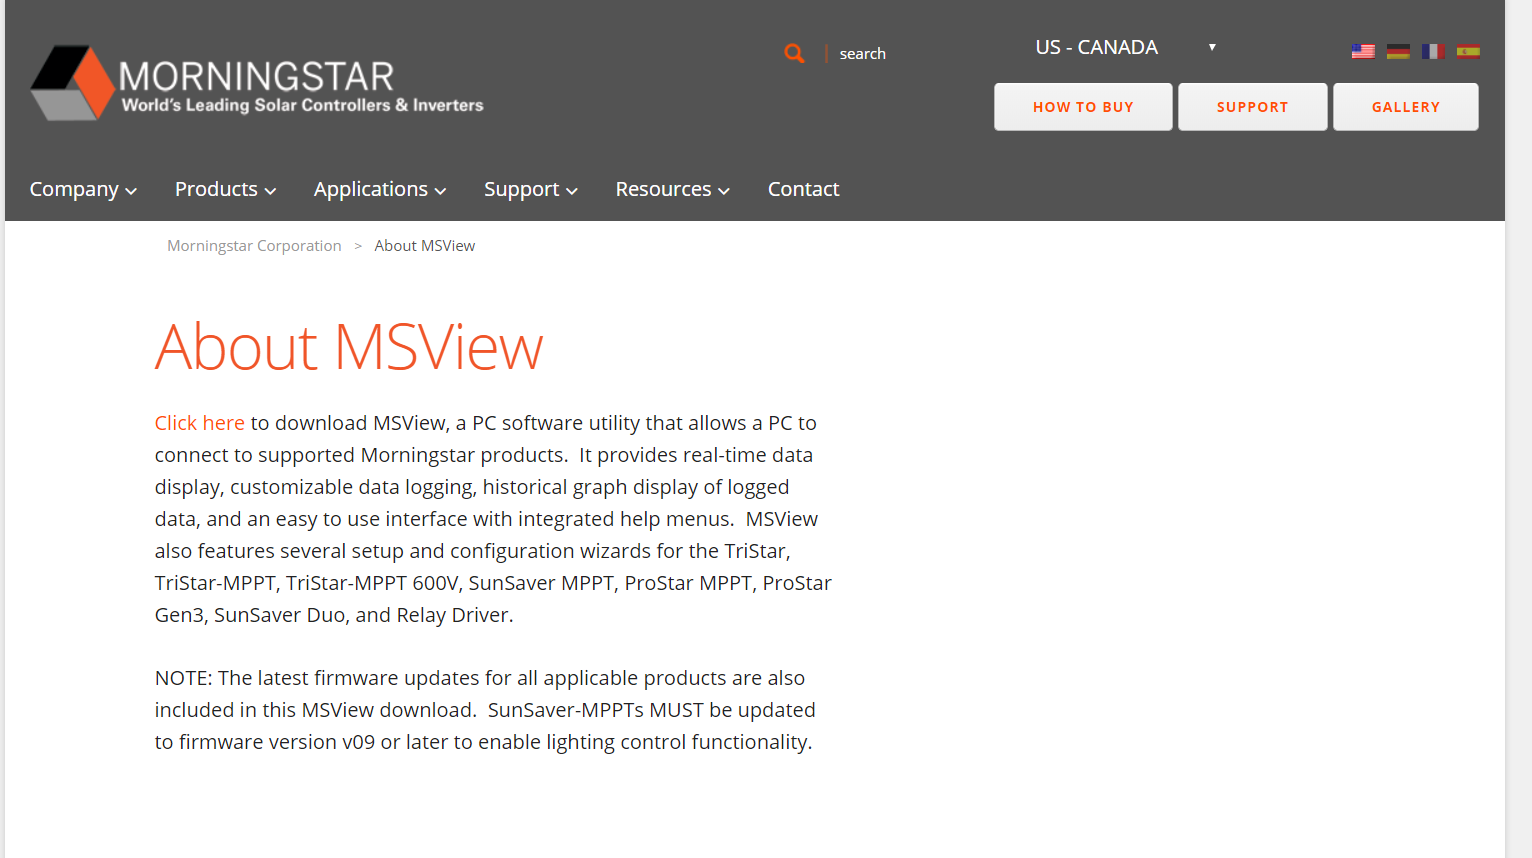
\includegraphics[width=\textwidth]{./graphics/tsmppt_troubleshooting/ms_1.png}
\caption{\label{fig:ms-website} Menu 1}
\end{figure}

\subsection{Step 2: Connecting the Morningstar}
If you’re using a RS-232 to USB serial connector to connect your PC, connect it now.

\subsection{Step 3: Powering the Morningstar}
Connect a 12V power supply to the battery terminal of the Tristar MPPT Charge Controller. It should draw approximately 189mA of current just for management.

\subsection{Step 4: Using MSView}
Open MSView.
Under Devices, select Search for Connected Devices. Your Tristar MPPT should show up under whatever virtual COM port you connected your RS-232 to USB connector to. Double-click it. You should see something like this appear.

\begin{figure}[h]
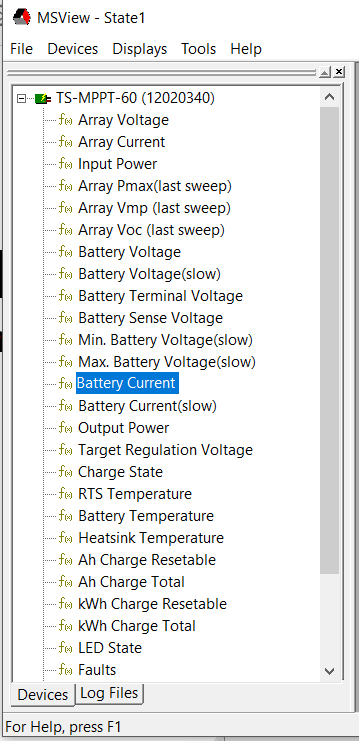
\includegraphics[width=0.7\columnwidth,angle=90,scale=0.75]{./graphics/tsmppt_troubleshooting/ms_2.png}
\caption{\label{fig:ms-website} First Menu upon initialization}
\end{figure}

\subsection{Step 5: Viewing Live Data}

Under Displays, select New. 
Select ‘State’ when a dialog box saying New Display appears and press OK.
Drag and drop whatever variables you want. Our Tristar MPPT can log:
\begin{itemize}
	\item Array Voltage (Array is shorthand for our solar panel array), 
	\item Array Current, Input Power (how much power our solar panels are producing), 
	\item Array Pmax, 
	\item Array Vmp, 
	\item Array Voc, 
	\item Battery Voltage (The Voltage of our Battery), 
	\item Battery Voltage (slow), 
	\item Battery Terminal Voltage, 
	\item Battery Sense Voltage (there’s a remote voltage sensor port on our Tristar MPPT that we can connect for safety), 
	\item Min. Battery Voltage (slow), 
	\item Max. Battery Voltage (slow), 
	\item Battery Current, 
	\item Battery Current(slow), 
	\item Output Power (how much power we’re consuming), 
	\item target regulation voltage, 
	\item charge state (Float, equalization, etc.), 
	\item RTS temperature, 
	\item Battery Temperature, 
	\item Heatsink Temperature, 
	\item Ah Charge Resetable, 
	\item Ah Charge Total, 
	\item kWh Charge Resetable, 
	\item kWh Charge Total, 
	\item LED State, Faults (did someone change the DIP switch?), 
	\item Faults Daily, 
	\item Alarms (did someone overcharge?), 
	\item Alarms Daily, 
	\item Hourmeter (how long have we been using this thing?),
	\item Settings Switches(the state of our DIP switch).
\end{itemize}

\subsection{Step 6: Programming the Tristar MPPT using MSView}

There are many different types of batteries: Lithium Ion, Lead-Acid, Lithium Polymer batteries, LiFePO4 batteries, etc. Each one of them requires its own different programming. The Tristar MPPT has 7 built-in programmable settings. To custom-program our Tristar MPPT to handle a battery, follow these steps:
\paragraph{}
Under Tools, click Tristar MPPT Setup Wizard. Read and click OK for both of the warnings against switching DIP switches while the power is applied.
\begin{figure}[!htb]
	\centering
	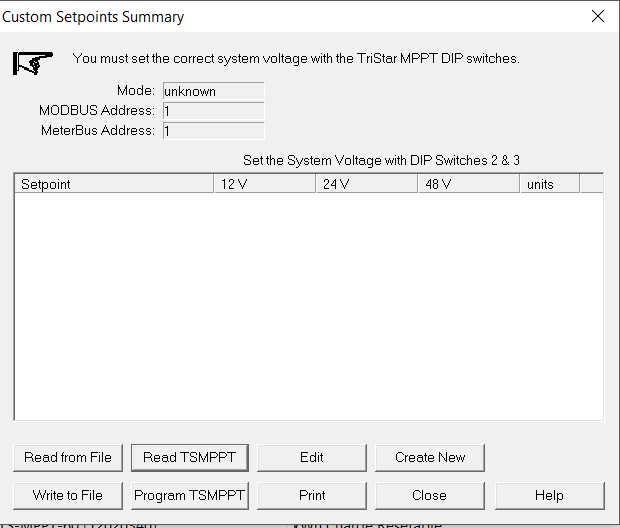
\includegraphics[width=0.6\columnwidth,scale=0.8]{./graphics/tsmppt_troubleshooting/ms_3.png}
	\caption{\label{fig:ts_setup_wizard} TSMPPT Setup Wizard}
\end{figure}

When on the screen that looks like Figure\ref{fig:ts_setup_wizard}, Click Read TSMPPT. Make sure it’s set to Solar Charge Control. If you’re using a serial connection, make sure you’re using the right COM port.
On our Tristar MPPT, the MODBUS address is 1.

% \begin{figure}%
	% \parbox{1.2in}{
		% 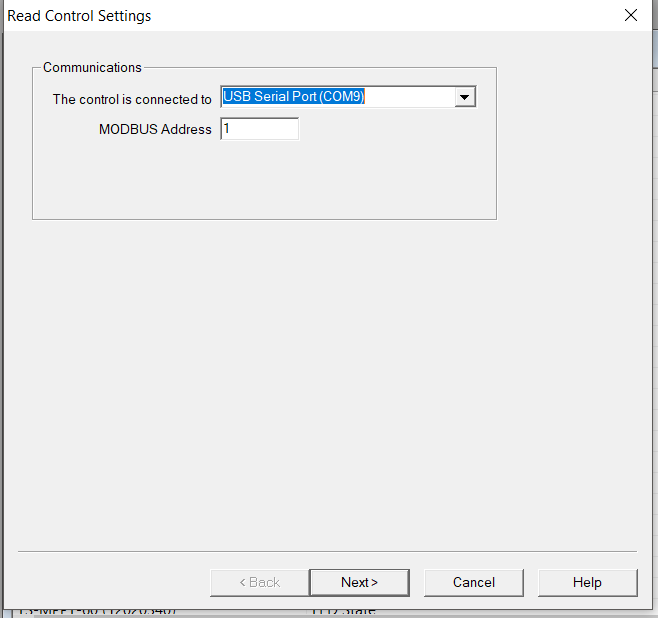
\includegraphics[width=0.6\columnwidth,scale=0.5]{./graphics/tsmppt_troubleshooting/ms_4.png}
		% \caption{First Figure}
	% }%
	% \qquad
	% \begin{minipage}{1.2in}%
		% 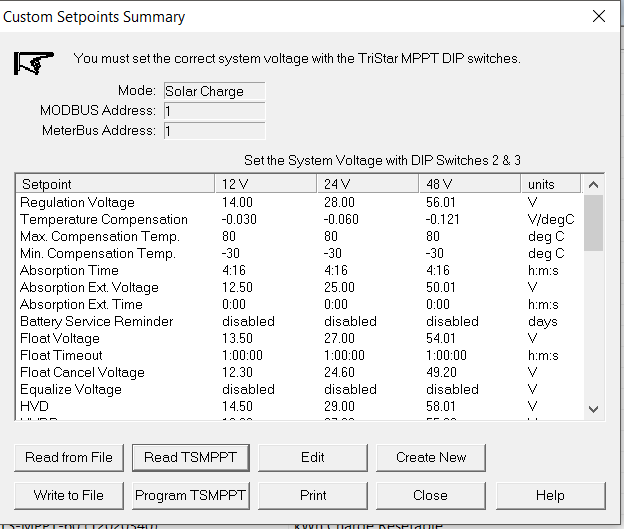
\includegraphics[width=\columnwidth,scale=0.7]{./graphics/tsmppt_troubleshooting/ms_5.png}
	% \end{minipage}%
	% \caption{Here are two figures side-by-side.}%
	% \label{fig:1figs}%
% \end{figure}

\begin{figure}[!htb]
	\centering
	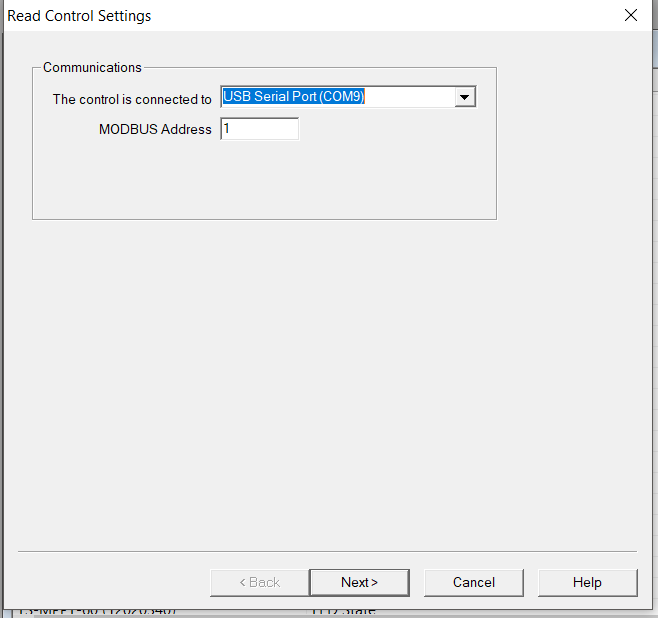
\includegraphics[width=\columnwidth]{./graphics/tsmppt_troubleshooting/ms_4.png}
	\caption{\label{fig:my-label} Communications settings}
\end{figure}

\begin{figure}[!htb]
	\centering
	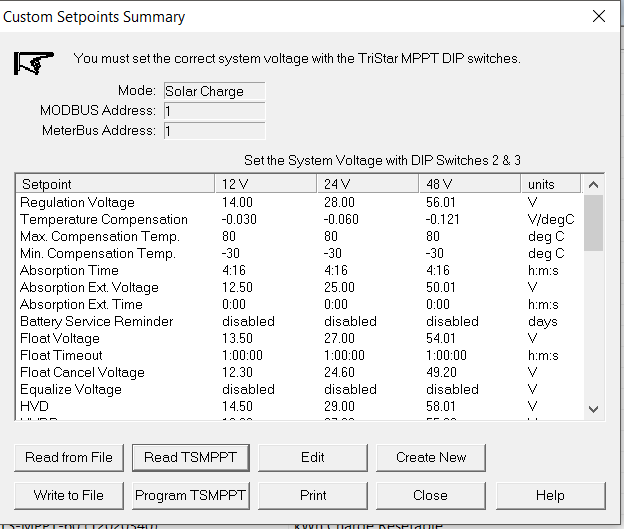
\includegraphics[width=\columnwidth]{./graphics/tsmppt_troubleshooting/ms_5.png}
	\caption{\label{fig:my-label} Tristar Morningstar Charge Settings Screen}
\end{figure}

The Setup wizard should look something like this afterwards if reading the settings was successful.

Read the settings you extracted from the Tristar MPPT first before you reprogram it. If the settings are not to your liking (i.e. the batteries will not charge properly), you can reprogram the Tristar MPPT. If you have a file already saved, click Read from File, and all your previously made changes will be loaded. 
If you don’t have a file made already, then click Edit. This will allow you to make your own custom settings.
You can change all these settings shown below:
  
 
\begin{figure}[!htb]
	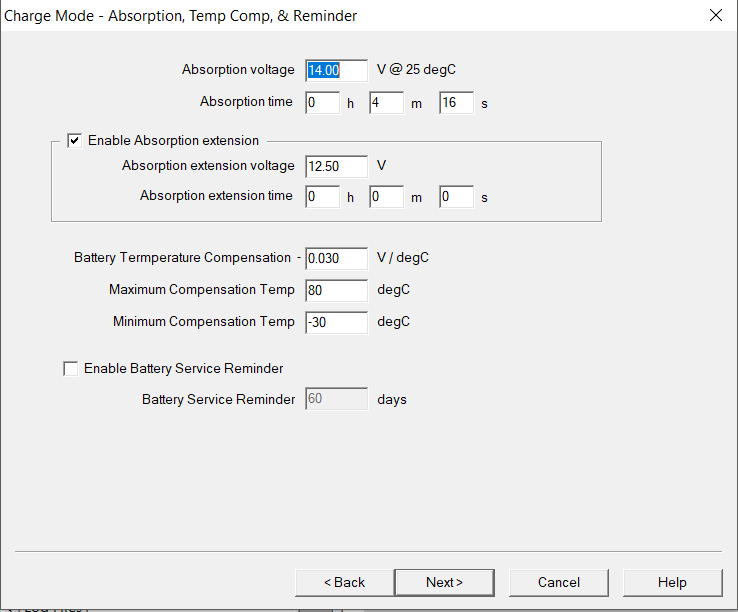
\includegraphics[width=\columnwidth,height=\textwidth,scale=0.5]{./graphics/tsmppt_troubleshooting/ms_6.png}
	\caption{\label{fig:settings-1} Absorption, Temperature Compensation, and Reminder Settings}
\end{figure}

\begin{figure}[!htb]
	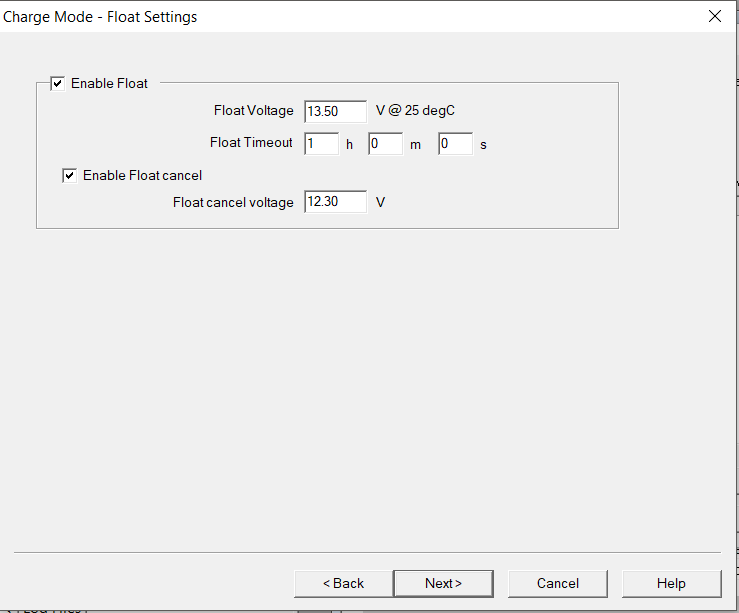
\includegraphics[width=\textwidth,height=\textwidth,scale=0.5]{./graphics/tsmppt_troubleshooting/ms_7.png}
	\caption{\label{fig:settings-2} Float Settings}
	
\end{figure}
\begin{figure}[!htb]
	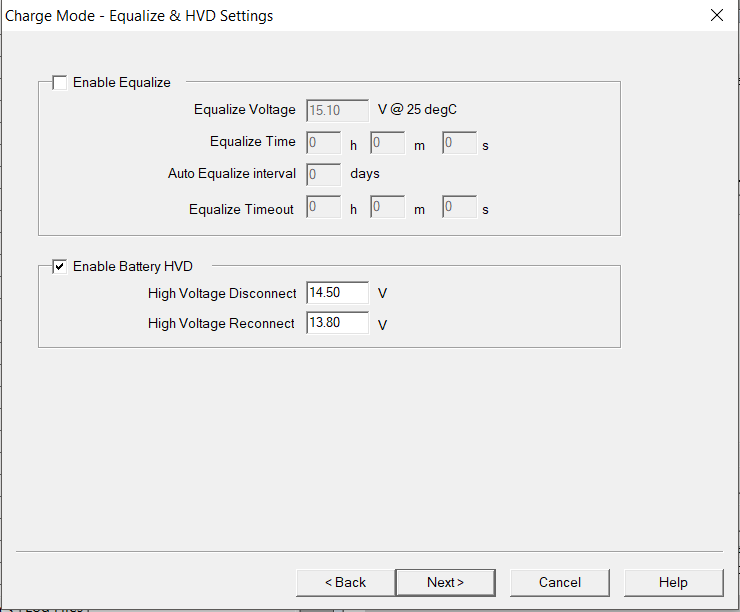
\includegraphics[width=\textwidth,height=\textwidth]{./graphics/tsmppt_troubleshooting/ms_8.png}
	\caption{\label{fig:settings-3} Equalize and HVD Settings}
\end{figure}
\begin{figure}[!htb]
	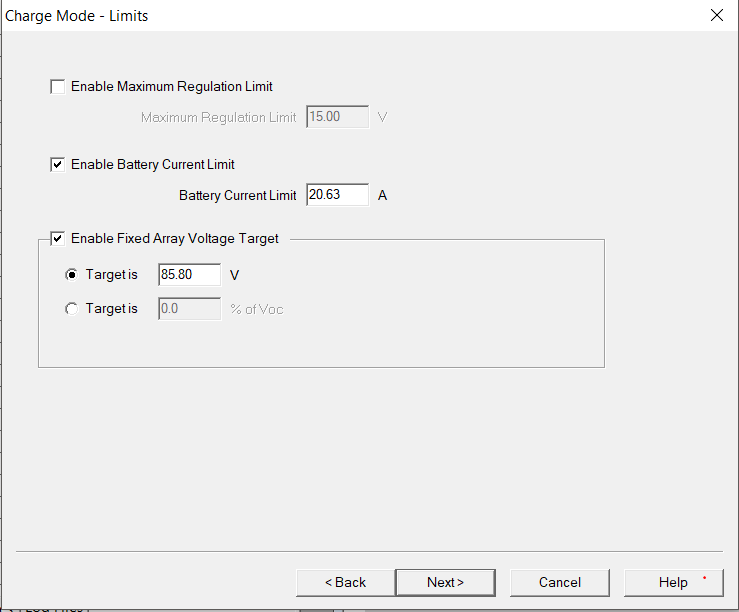
\includegraphics[width=\textwidth,height=\textwidth]{./graphics/tsmppt_troubleshooting/ms_9.png}
	\caption{\label{fig:settings-4} Limits Settings}
\end{figure}
\begin{figure}[!htb]
	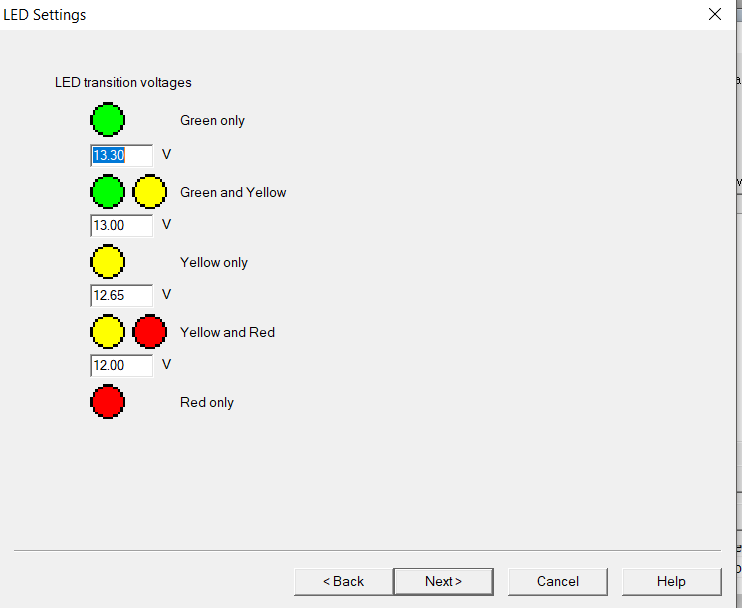
\includegraphics[width=\textwidth,height=\textwidth]{./graphics/tsmppt_troubleshooting/ms_10.png}
	\caption{\label{fig:settings-5} LED Settings}
\end{figure}
\begin{figure}[!htb]
	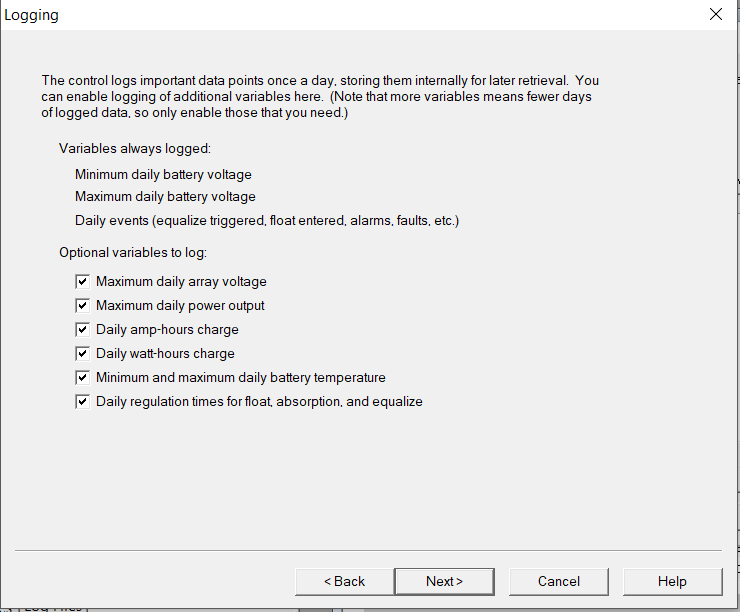
\includegraphics[width=\textwidth,height=\textwidth]{./graphics/tsmppt_troubleshooting/ms_11.png}
	\caption{\label{fig:settings-6} Logger Settings}
\end{figure}
\begin{figure}[!htb]
	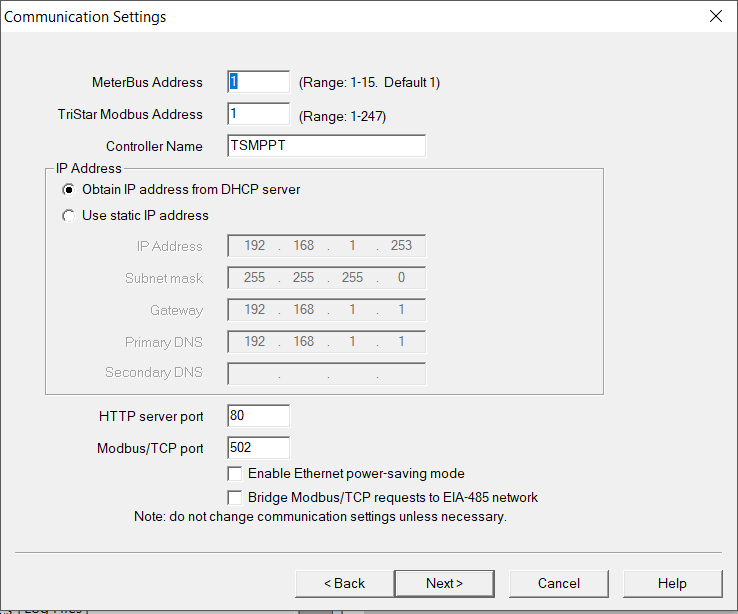
\includegraphics[width=\textwidth,height=\textwidth]{./graphics/tsmppt_troubleshooting/ms_12.png}
	\caption{\label{fig:settings-7} Commmunication Settings}
\end{figure}
\begin{figure}[!htb]
	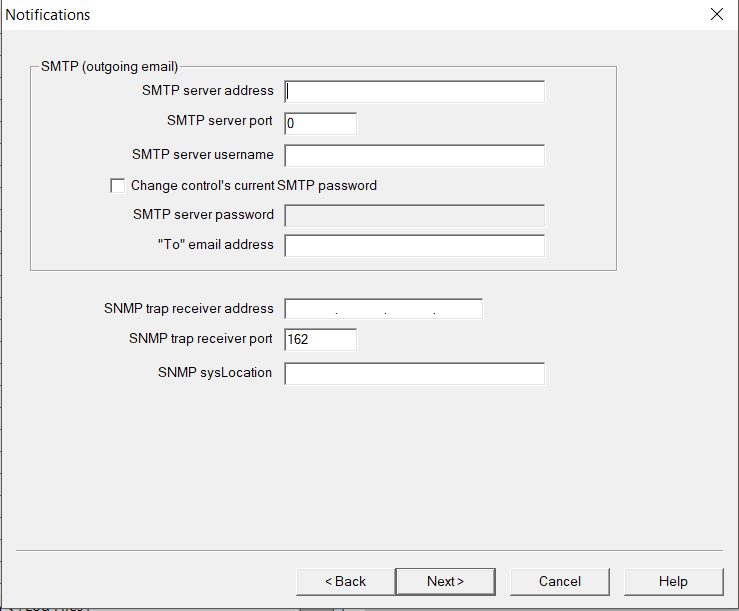
\includegraphics[width=\textwidth,height=\textwidth]{./graphics/tsmppt_troubleshooting/ms_13.png}
	\caption{\label{fig:settings-8} Mail Server Settings (TCP Exclusive)}
\end{figure}
\begin{figure}[!htb]
	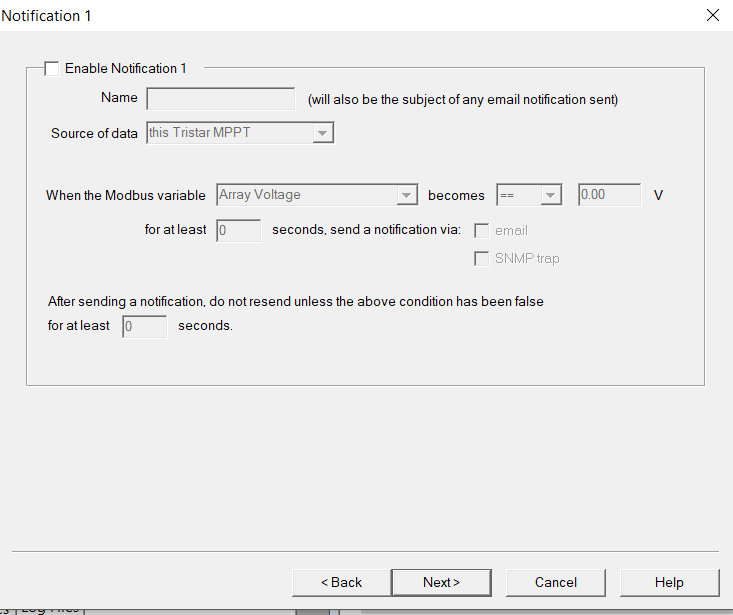
\includegraphics[width=\textwidth,height=\textwidth]{./graphics/tsmppt_troubleshooting/ms_14.png}
	\caption{\label{fig:settings-9} Notification 1}
\end{figure}
\begin{figure}[!htb]
	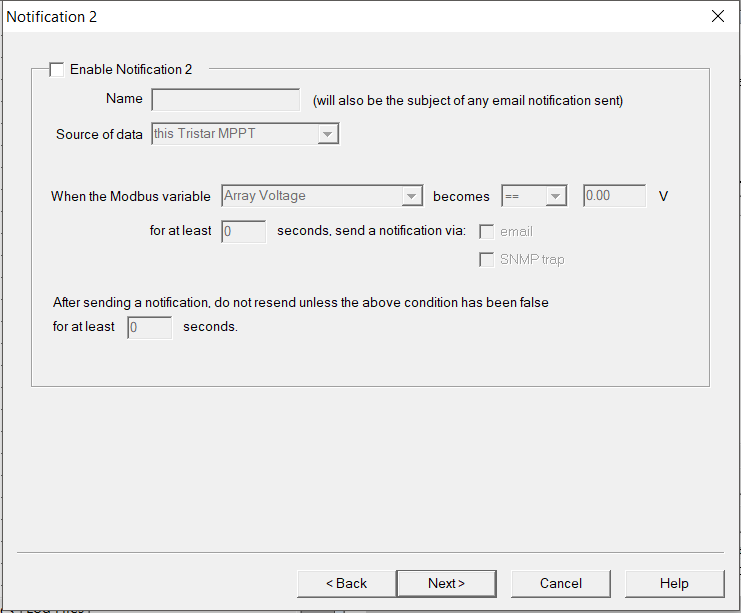
\includegraphics[width=\textwidth,height=\textwidth]{./graphics/tsmppt_troubleshooting/ms_15.png}
	\caption{\label{fig:settings-10} Notification 2}
\end{figure}
\begin{figure}[!htb]
	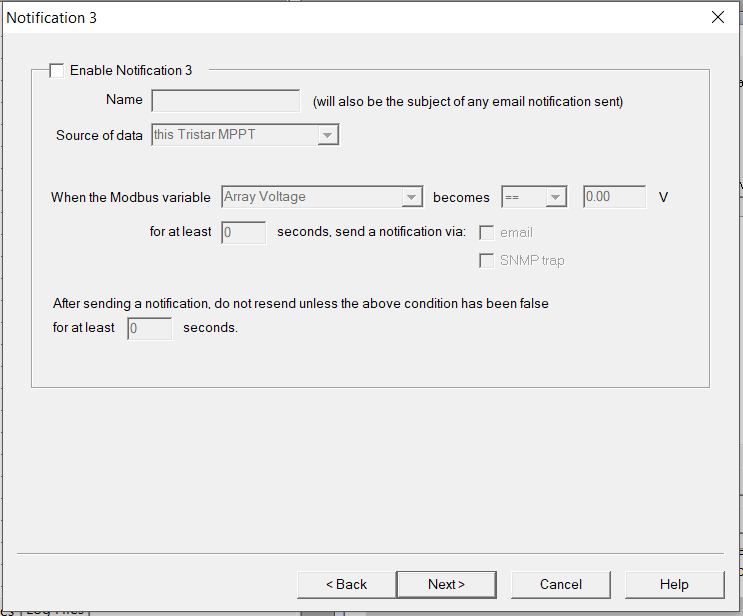
\includegraphics[width=\textwidth,height=\textwidth]{./graphics/tsmppt_troubleshooting/ms_16.png}
	\caption{\label{fig:settings-11} Notification 3}
\end{figure}
\begin{figure}[!htb]
	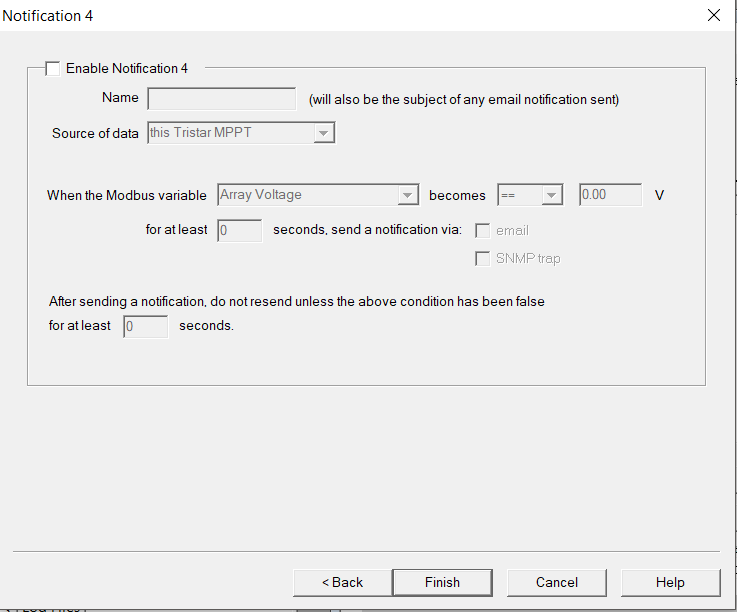
\includegraphics[width=\textwidth,height=\textwidth]{./graphics/tsmppt_troubleshooting/ms_17.png}
	\caption{\label{fig:settings-12} Notification 4}
\end{figure}
\begin{figure}[!htb]
	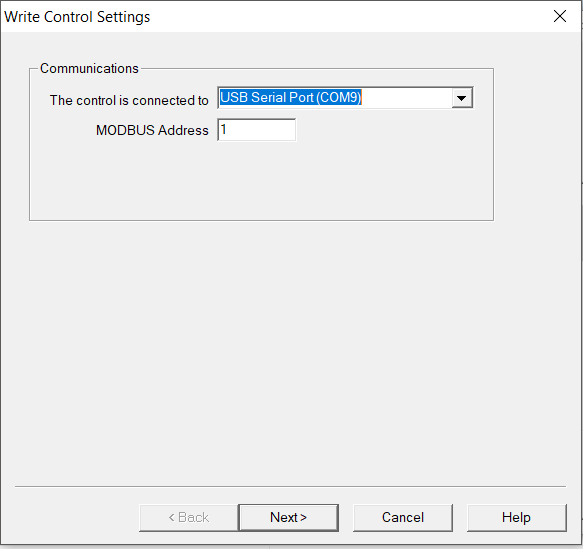
\includegraphics[width=\textwidth,height=\textwidth]{./graphics/tsmppt_troubleshooting/ms_18.png}
	\caption{\label{fig:settings-13} Write Control Communication Settings}
\end{figure}
\begin{figure}[!htb]
	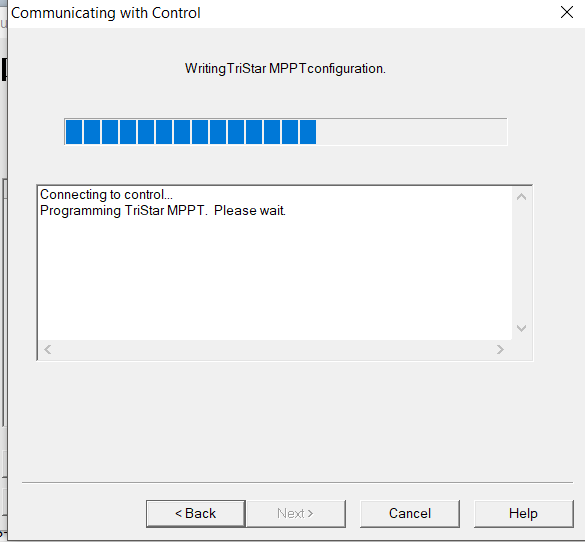
\includegraphics[width=\textwidth,height=\textwidth]{./graphics/tsmppt_troubleshooting/ms_19.png}
	\caption{\label{fig:settings-14} Writing Settings to the Tristar Screen}
\end{figure}

\paragraph{}
Once all of your changes are made, you can save it to a file, just in case you need to reprogram the Tristar MPPT. Save it by using Write to File.

Once you have your settings loaded, you need to program the Tristar MPPT. Click Program TSMPPT, and make sure the COM port is correct.

Now, your Tristar should be ready to be used with your batteries!

\subsection{Final Step}
Oh, one more thing! If you want to use custom charging settings, DIP switches 4,5, and 6 must be switched on! That’s how the custom settings work! It even says so in MSView! \\
Also, this is a CHARGE CONTROLLER! It won’t manage all your batteries for you! You must use a BMS system for that. Luckily, we have one. I’ve got a separate document for that. It can help you balance out the charges on your batteries so that every battery has an even charge, and none of them use too many life cycles at the same time.
 \\




\chapter{Datasheets}

\section{Sensor datasheet}
\subsection{TSL2591}
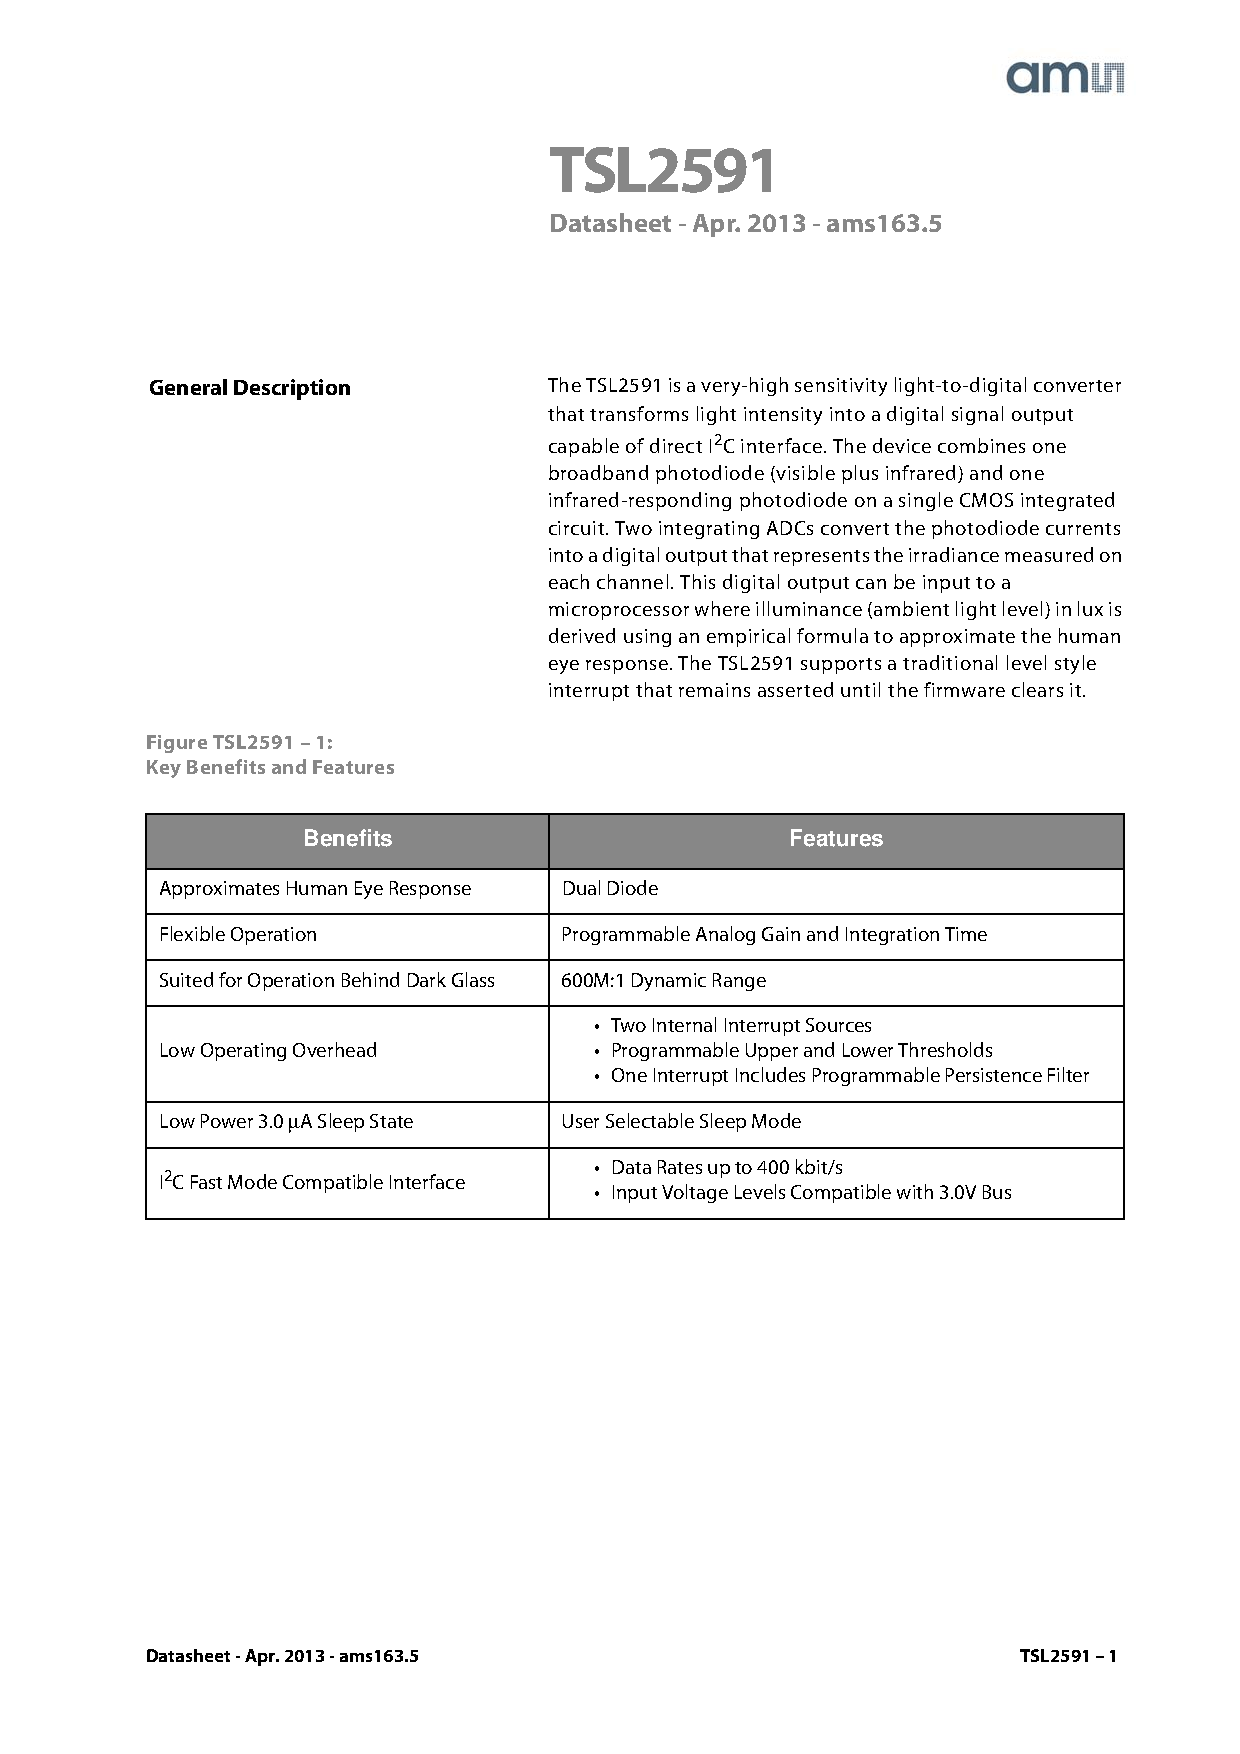
\includepdf[pages=-]{"./datasheets/Light Sensors/TSL2591.pdf"}
\section{Microcontroller Datasheets}

\section{Raspberry Pi 3B+ Schematic}
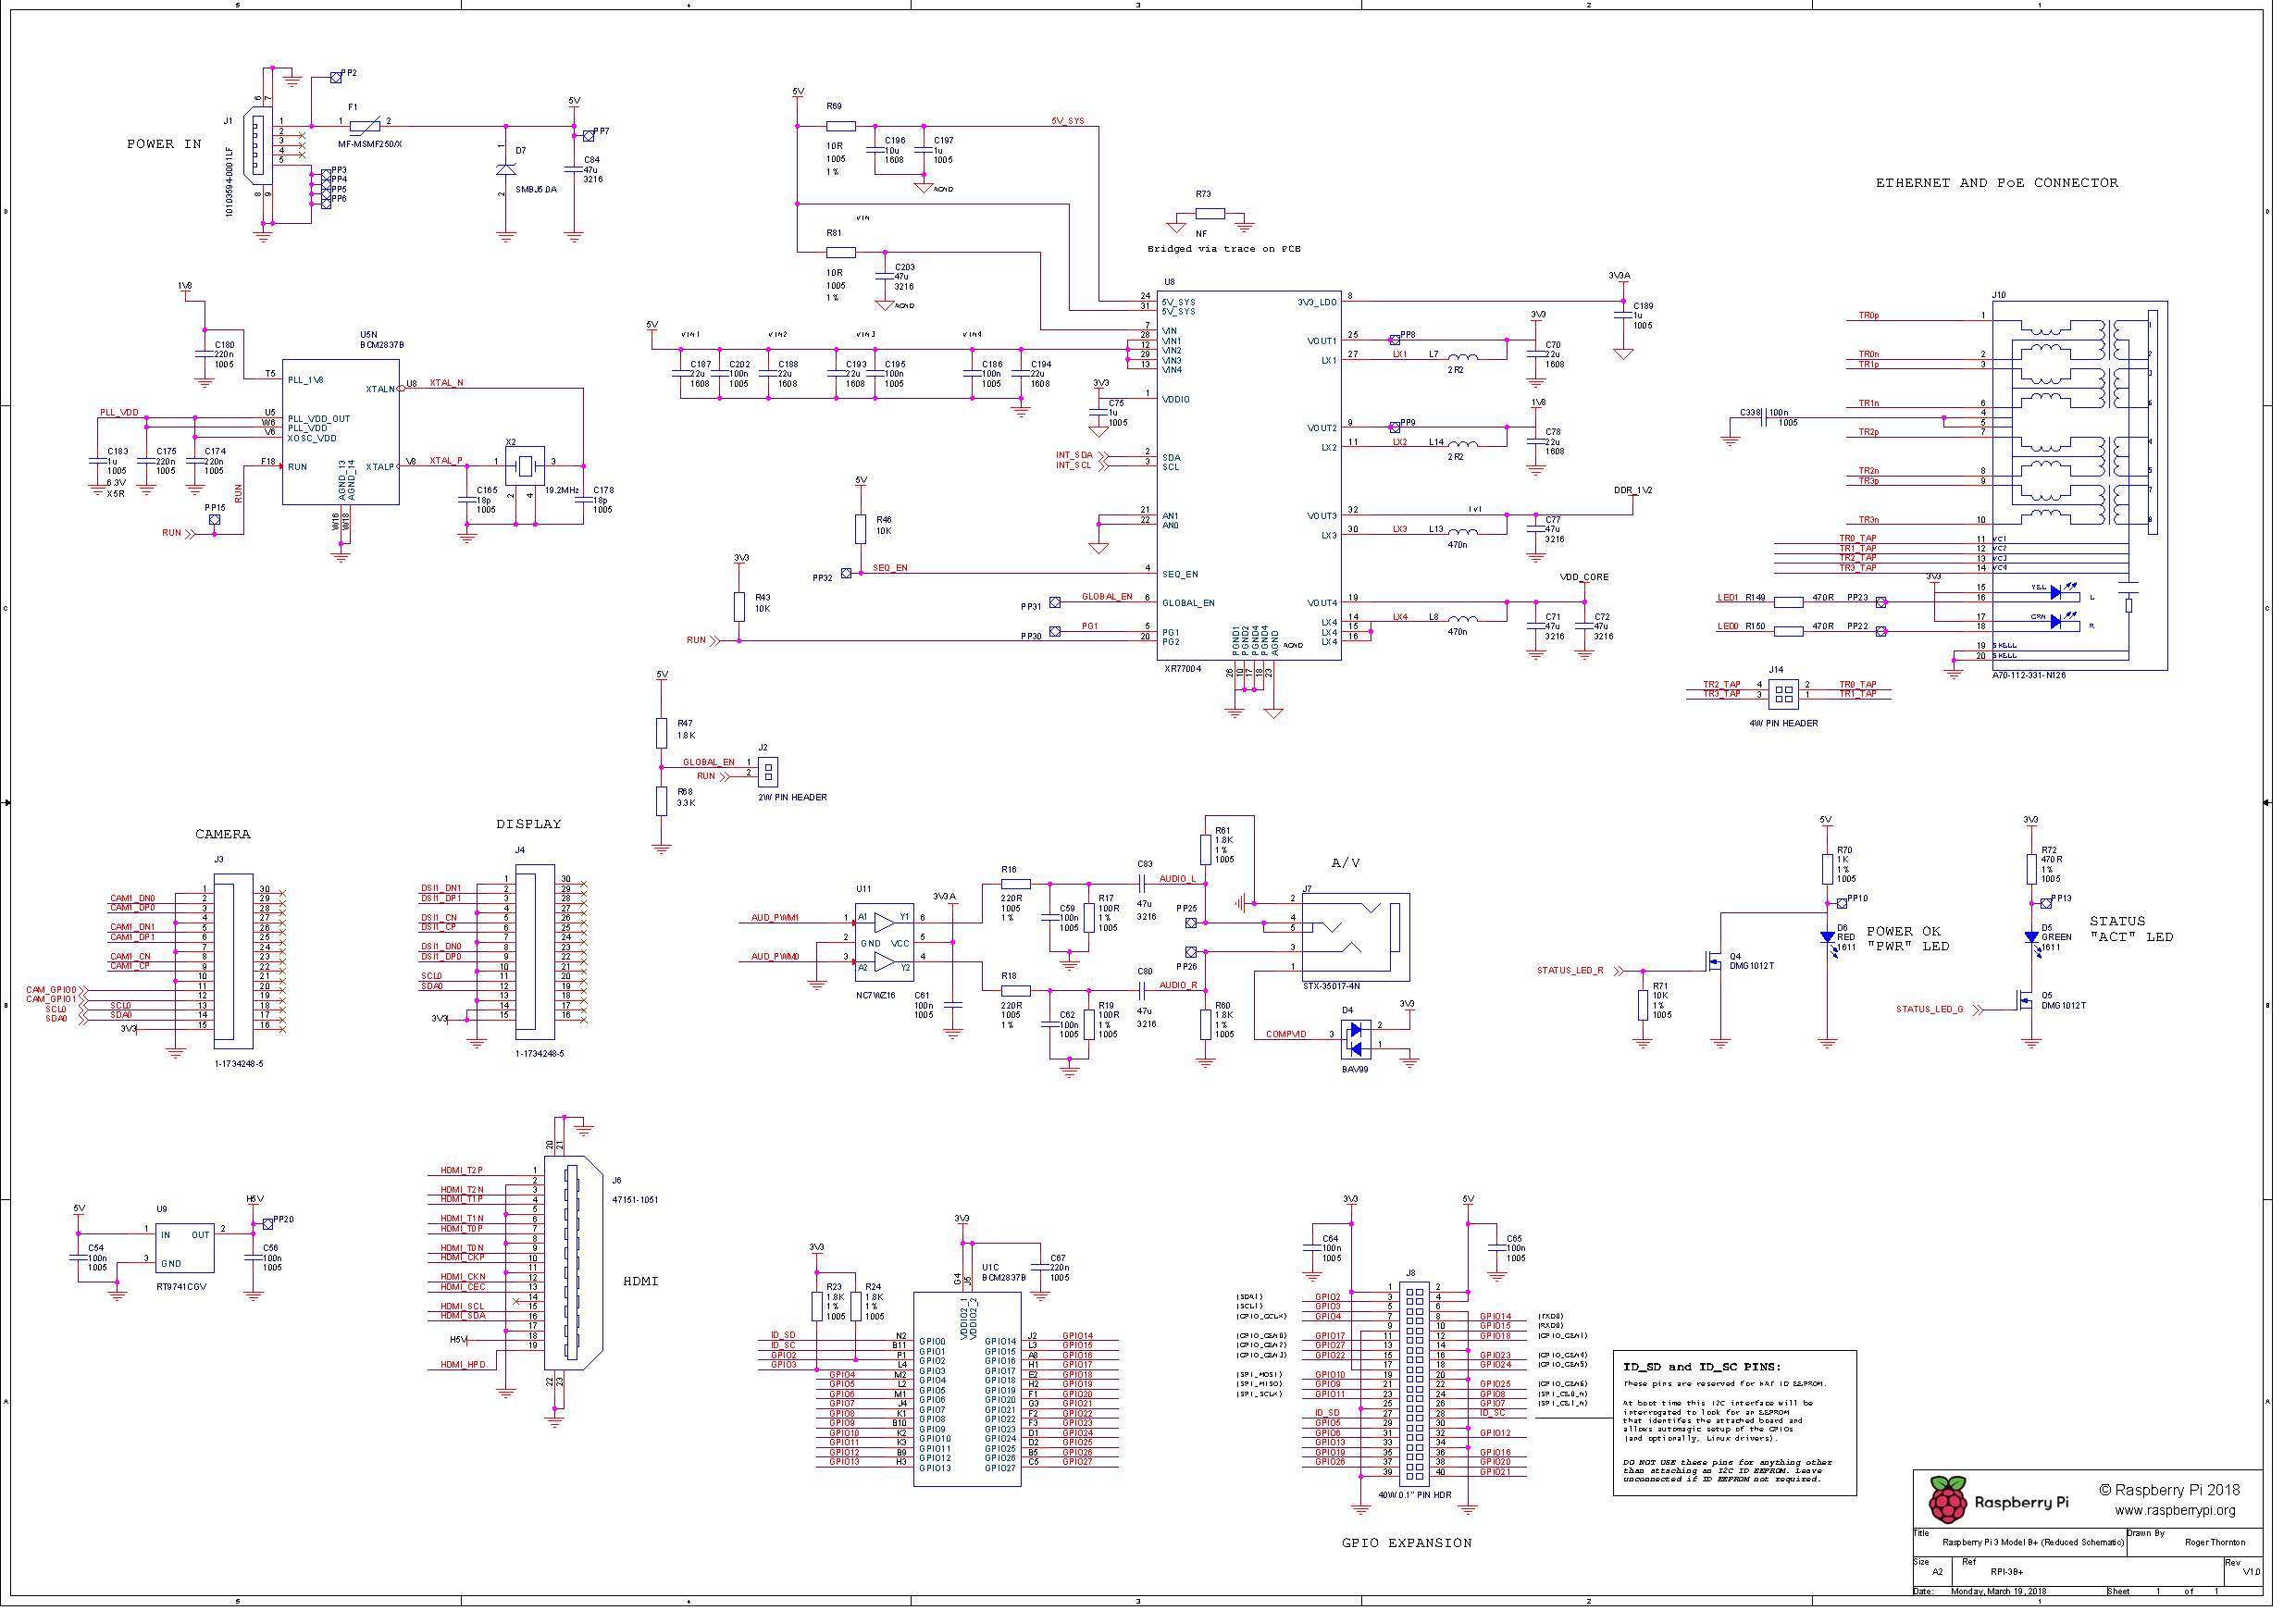
\includepdf[pages=-]{"./datasheets/Microcontrollers/raspberry_pi_3Bplus_sch.pdf"}

\section{Tristar MPPT Operator's Manual}
\includepdf[pages=-]{"./datasheets/MPPT Controller/150V-TS-MPPT-Operators-Manual.pdf"}

\section{Solar Panel Datasheet}
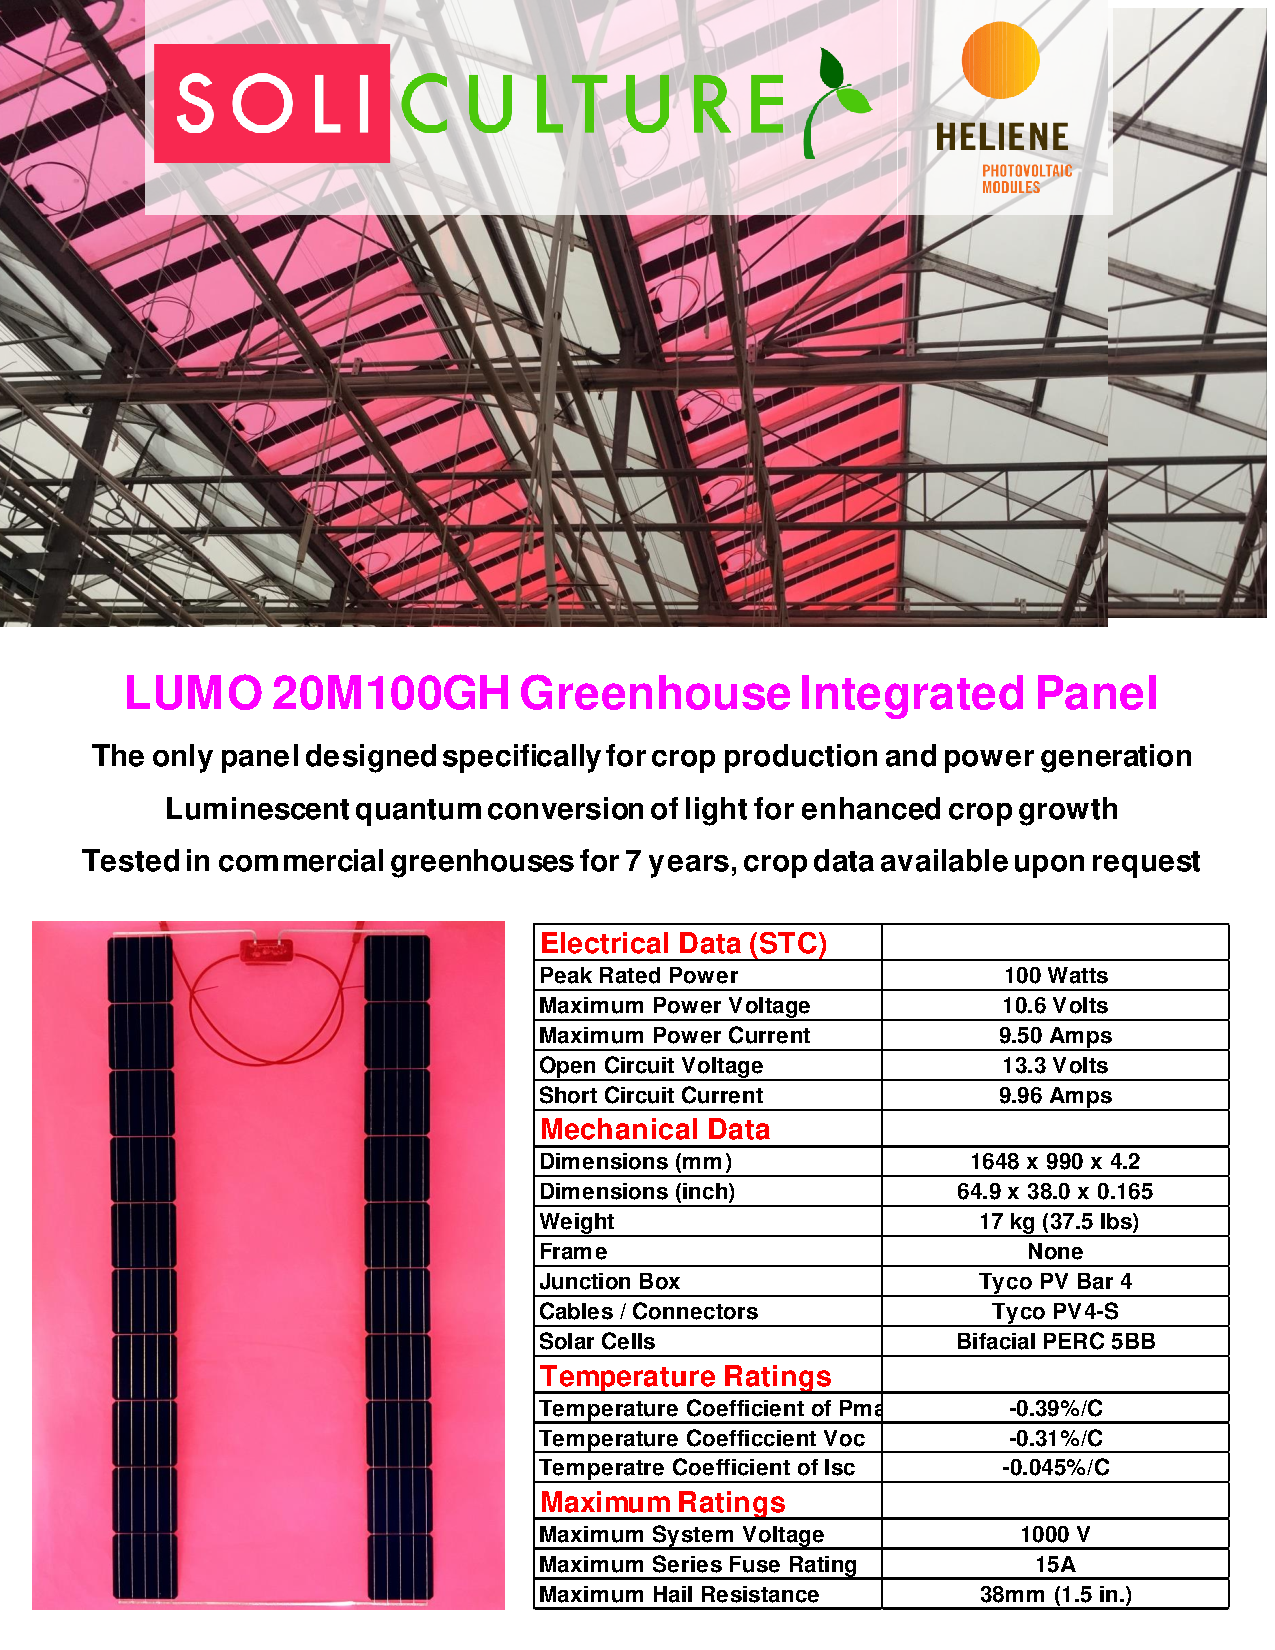
\includepdf[pages=-]{"./datasheets/MPPT Controller/Datasheet-LUMO20M100GH - Solar Panel.pdf"}

\section{Battery Datasheet}
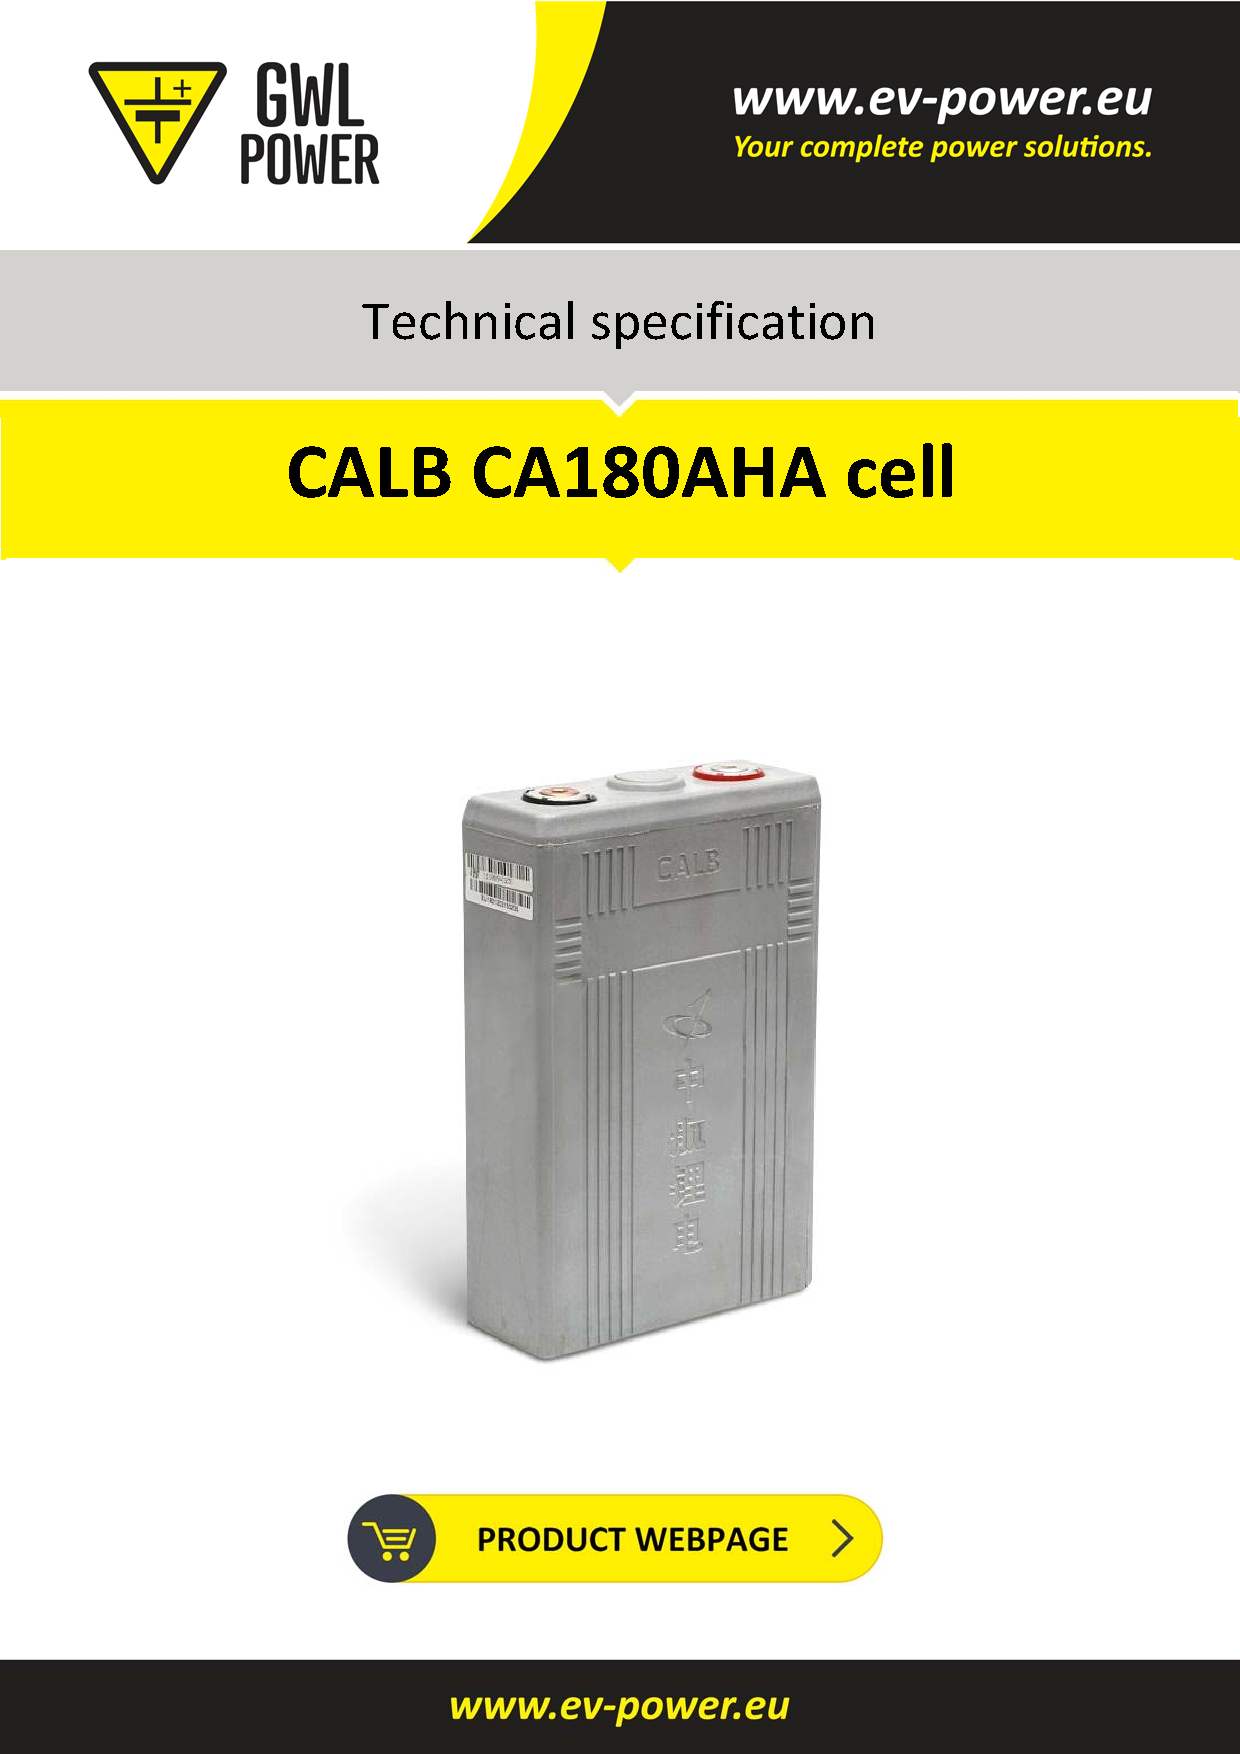
\includepdf[pages=-]{"./datasheets/Batteries/CALB_battery.pdf"}

\end{document}